\documentclass[11pt,a4paper]{article}

% ============================================================
% Packages
% ============================================================

\usepackage[utf8]{inputenc}
\usepackage[T1]{fontenc}
\usepackage{lmodern}

\usepackage[
    a4paper,
    top=2.3cm,
    bottom=2.3cm,
    left=2.5cm,
    right=2.5cm
]{geometry}

\usepackage{graphicx}
\usepackage{booktabs}
\usepackage{array}
\usepackage{tabularx}
\usepackage{amsmath}
\usepackage{amssymb}
\usepackage{float}
\usepackage{enumitem}
\usepackage{setspace}
\usepackage{parskip}
\usepackage{xcolor}
\usepackage{hyperref}
\usepackage{fancyhdr}
\usepackage{lastpage}
\usepackage{titlesec}

% ============================================================
% General Formatting
% ============================================================

\setstretch{1.15}

\setlength{\parindent}{0pt}
\setlength{\parskip}{6pt}
\setlength{\headheight}{14pt}

\hypersetup{
    colorlinks=true,
    linkcolor=black,
    citecolor=black,
    urlcolor=blue
}

\titleformat{\section}
{\large\bfseries}
{\thesection.}
{0.6em}
{}

\titleformat{\subsection}
{\normalsize\bfseries}
{\thesubsection}
{0.6em}
{}

\titleformat{\subsubsection}
{\normalsize\bfseries}
{\thesubsubsection}
{0.6em}
{}

% ============================================================
% Main Report Header / Footer
% ============================================================

\fancypagestyle{main}{
    \fancyhf{}
    \fancyhead[L]{FN6809 Linear Financial Models}
    \fancyhead[R]{Group 10}
    \fancyfoot[C]{Page \thepage}
    \renewcommand{\headrulewidth}{0.4pt}
    \renewcommand{\footrulewidth}{0pt}
}

% ============================================================
% Document
% ============================================================

\begin{document}

% ============================================================
% PAGE 1 - COVER PAGE
% ============================================================

\begin{titlepage}
\thispagestyle{empty}

\begin{center}

\vspace*{0.8cm}


\includegraphics[width=0.82\textwidth]{nbs_logo.jpg}

\vspace{1.8cm}

{\LARGE\bfseries Exploring the Drivers of U.S. Domestic Airline Fares}

\vspace{0.25cm}

{\large An Exploratory Multiple Regression Analysis}

\vspace{0.8cm}

{\large\bfseries Group 10}

\vspace{1.4cm}

\begin{tabular}{>{\bfseries}p{4.2cm} p{8.5cm}}
Course Code: & FN6809 \\[0.45cm]
Course Title: & Linear Financial Models \\[0.45cm]
Lecturer: & Assoc Prof Wu Yuan \\[0.45cm]
Date Submitted: & 31 October 2026 \\
\end{tabular}

\vspace{1.4cm}

{\large\bfseries Student Name / ID}

\vspace{0.5cm}

\begin{tabular}{r l l}
1. & Fu Yuxuan (G) & \\[0.15cm]
2. & Koh Chen Yang (G2601860H) & \\[0.15cm]
3. & Ma Qimin (G) & \\[0.15cm]
4. & Verma Aditya Aryan (G) & \\[0.15cm]
5. & Yin Qiuhao (G) & \\[0.15cm]
6. & Zhu Jingyu (G) & \\
\end{tabular}

\vfill

\end{center}
\end{titlepage}

% ============================================================
% DECLARATION
% ============================================================

\clearpage
\thispagestyle{empty}

\vspace*{0.8cm}

{\large\bfseries Declaration}

\vspace{0.5cm}

We declare that this assessment item is our own work, except where acknowledged, and has not been submitted for academic credit elsewhere, and acknowledge that the assessor of this item may, for the purpose of assessing this item:

\begin{itemize}[leftmargin=2em]
    \item reproduce this assessment item and provide a copy to another member of the University; and/or,
    \item communicate a copy of this assessment item to a plagiarism checking service (which may then retain a copy of the assessment item on its database for the purpose of future plagiarism checking).
\end{itemize}

\vspace{0.6cm}

We certify that we have read and understood the University Academic Standing and Grading System in respect of Student Honour Code.

\vspace{1.2cm}

\begin{tabularx}{\textwidth}{X X}
Signed: \hrulefill & Date: \hrulefill \\[0.75cm]
Signed: \hrulefill & Date: \hrulefill \\[0.75cm]
Signed: \hrulefill & Date: \hrulefill \\[0.75cm]
Signed: \hrulefill & Date: \hrulefill \\[0.75cm]
Signed: \hrulefill & Date: \hrulefill \\[0.75cm]
Signed: \hrulefill & Date: \hrulefill \\
\end{tabularx}

% ============================================================
% CONTENTS
% ============================================================

\clearpage
\pagestyle{empty}

\tableofcontents

\clearpage
\setcounter{page}{1}
\pagestyle{main}

% ============================================================
% EXECUTIVE SUMMARY
% ============================================================

\clearpage
\setcounter{page}{1}
\pagestyle{main}

\section*{Executive Summary}
\addcontentsline{toc}{section}{Executive Summary}

This study investigates which observable itinerary, carrier, purchase, and geographic characteristics are most useful in explaining variation in U.S. domestic airline ticket fares. Using the June 2026 U.S. Bureau of Transportation Statistics DB1C Ticket dataset, a reproducible random sample of 100,000 tickets was drawn from more than 13.8 million records. After excluding tax-only, nominal-fare, and incomplete observations, 90,086 regular positive-fare tickets were retained for analysis.

Eight predictor blocks were considered: itinerary distance, number of ticket coupons, round-trip status, carrier structure, purchase window, reporting carrier, itinerary geography, and origin state. The initial level-fare OLS model exhibited substantial heteroskedasticity and right-skewed residuals. A logarithmic transformation of ticket fare improved the residual structure, while empirical weighted least squares further reduced unequal variance. OLS with White heteroskedasticity-robust standard errors was also used as a robustness benchmark and produced broadly similar substantive conclusions.

The final model retains all eight predictor blocks. Travel distance and itinerary complexity are positively associated with fare: an additional 100 itinerary miles is associated with approximately a 1.58\% higher fare, while each additional ticket coupon is associated with approximately a 1.32\% increase. Round-trip tickets are associated with approximately 55.20\% higher total ticket amounts than comparable one-way tickets, while \texttt{OnLine = 0} itineraries are associated with approximately 10.40\% higher fares. Relative to the \texttt{21AP} purchase-window category, the \texttt{2290} and \texttt{91UP} categories are associated with fares approximately 26.52\% and 27.19\% lower, respectively. Material conditional differences are also observed across carriers and origin states.

The model was evaluated using an independent 50\% validation sample. The selected eight-block specification achieved a validation mean squared prediction error of 0.2061 on the log-fare scale, only approximately 1.5\% above its model-building MSE. Its adjusted \(R^2\) declined only modestly from 0.573 in the model-building sample to 0.568 in validation, while the economically important coefficients remained broadly stable. A seven-block alternative excluding \texttt{Coupons} produced almost identical predictive performance, but \texttt{Coupons} remained stable and statistically significant after refinement and validation and added only one parameter. It was therefore retained because the study places emphasis on explanatory value as well as predictive performance.

The final model is also translated into a practical conditional fare benchmark. The median observed fare is \$388.40 compared with a median model-implied benchmark of \$378.17, with a median percentage gap of only -0.26\%. Approximately 48\% of tickets fall within 25\% of their benchmark, while the remainder can be identified as relatively high- or low-priced conditional on their observable characteristics. The benchmark is not intended to reproduce airline revenue-management systems or establish a uniquely correct fare; rather, it provides a transparent reference point for interpreting ticket prices after accounting for systematic differences across itineraries.

Overall, the analysis shows that observable itinerary, purchase, carrier, and geographic characteristics explain a meaningful portion of cross-sectional airline-fare variation. Despite remaining heteroskedasticity and unobserved pricing factors, the final model is statistically stable, interpretable, and useful both for explaining fare differences and for constructing a practical conditional fare benchmark.

% ============================================================
% SECTION 1 - INTRODUCTION AND RESEARCH OBJECTIVE
% ============================================================

\clearpage

\section{Introduction and Research Objective}

\subsection{Motivation}

Airline ticket prices vary substantially across passengers and itineraries, even within the same market period. A fare that appears high in absolute terms may be reasonable for a long or complex itinerary, while a lower fare may still be expensive relative to tickets with similar characteristics. Consequently, comparing ticket prices without accounting for differences in itinerary structure, purchase timing, carrier, and geography can be misleading.

This makes airline fares a natural application for multiple regression. Rather than asking only whether fares differ across tickets, regression allows these differences to be examined after controlling simultaneously for multiple observable characteristics. For example, the relationship between travel distance and fare can be assessed while holding carrier and purchase conditions fixed, while carrier differences can be examined after controlling for itinerary characteristics.

An interpretable model is particularly valuable in this setting. Airline pricing is influenced by many interacting factors, and a highly complex predictive model may achieve good predictive performance without clearly explaining why predicted fares differ. In contrast, a linear regression framework provides transparent estimates of how observable ticket characteristics are associated with higher or lower fares.

The practical relevance extends beyond coefficient interpretation. Once systematic differences in fares are accounted for, the fitted model can provide a reference point for evaluating individual tickets. A ticket priced substantially above the model-implied fare may be considered relatively expensive compared with tickets sharing similar observable characteristics, whereas a ticket priced below the benchmark may be considered relatively inexpensive.

The objective is therefore not to reproduce an airline's internal pricing algorithm, but to develop a transparent statistical framework that explains a meaningful portion of observed fare variation and translates those relationships into a practical fare benchmark.

\subsection{Research Objective}

This study investigates cross-sectional variation in U.S. domestic airline ticket fares using an interpretable multiple regression framework.

The primary research question is:

\begin{quote}
\textbf{Which observable itinerary, carrier, purchase, and geographic characteristics are most useful in explaining variation in U.S. domestic airline ticket fares?}
\end{quote}

To address this question, the study has three related objectives:

\begin{enumerate}
    \item identify the observable ticket characteristics that contribute meaningfully to explaining fare variation;
    \item quantify the direction and economic magnitude of the associations between these characteristics and ticket fares; and
    \item assess whether the resulting model can provide a useful benchmark for identifying relatively high- or low-priced tickets after controlling for observable characteristics.
\end{enumerate}

The emphasis is therefore placed not only on statistical fit, but also on model interpretability, stability, and practical usefulness.

\subsection{Scope and Interpretation}

The analysis is exploratory and observational. It examines differences across U.S. domestic airline tickets observed within a common reporting period rather than changes in airfare levels over time.

Accordingly, the estimated regression coefficients are interpreted as conditional associations rather than causal effects. For example, a positive carrier coefficient indicates that tickets associated with that carrier tend to have higher fares after controlling for the other variables included in the model; it does not imply that the carrier itself causes fares to increase.

The model also does not attempt to capture every determinant of airline pricing. Some important factors, such as real-time seat availability, detailed fare restrictions, loyalty status, and contemporaneous competitive conditions, may not be fully observed in the available data.

The aim is instead to explain the systematic component of fare variation that can be linked to observable ticket characteristics. A model that remains statistically stable, interpretable, and useful for benchmarking can still provide meaningful insight even when a substantial portion of individual ticket-price variation remains unexplained.

% ============================================================
% SECTION 2 - DATA AND VARIABLE CONSTRUCTION
% ============================================================

\section{Data and Variable Construction}

\noindent\textit{Code reference: Notebook 01 (\texttt{01\_data\_preparation.ipynb}).}

\subsection{Data Source and Reproducible Sampling}

The study uses the June 2026 U.S. Bureau of Transportation Statistics DB1C Ticket dataset. The dataset contains ticket-level information on complete domestic itineraries, including fares, carriers, itinerary structure, purchase characteristics, distance, and geography.

The raw June 2026 Ticket file contains 13,822,006 observations and is approximately 2.52 GB in size. Estimating the exploratory models on every observation would add substantial computational cost without being necessary for the purpose of this project. A reproducible random sample of 100,000 ticket records is therefore drawn from the complete file.

To avoid dependence on the ordering of the source CSV, the raw file is processed sequentially in chunks and each observation is assigned a random priority using a fixed random seed of 42. After the entire file has been processed, the 100,000 observations with the smallest random priorities are retained. This procedure allows observations throughout the source file to enter the analysis sample while avoiding the need to load the entire dataset into memory.

\subsection{Fare-Quality Screening}

Initial inspection reveals a distinct group of records that are not representative of conventionally priced commercial tickets. Rather than removing observations using an arbitrary threshold on the total ticket amount, fare quality is assessed using the non-tax component of the ticket:

\[
\texttt{AmountExclTax} = \texttt{TotalAmount} - \texttt{TaxAmount}.
\]

Three data-quality issues are identified.

First, 9,339 sampled observations have a zero non-tax fare component, meaning that the reported total ticket amount consists entirely of taxes. These records account for 9.339\% of the 100,000-ticket sample and form a clearly distinct fare population.

Second, 569 observations contain a positive but nominal non-tax fare component of no more than \$0.02. The concentration of observations at values such as \$0.01 and \$0.02 suggests a discrete pricing convention or special ticket structure rather than the lower tail of ordinary continuous fare variation.

Third, six observations have missing fare information.

The records are therefore classified as follows:

\begin{itemize}
    \item \textbf{Missing}: \texttt{AmountExclTax} is missing;
    \item \textbf{Tax-only}: \texttt{AmountExclTax} equals zero;
    \item \textbf{Nominal fare}: \texttt{AmountExclTax} is positive but no greater than \$0.02;
    \item \textbf{Regular positive fare}: \texttt{AmountExclTax} exceeds \$0.02.
\end{itemize}

Table~\ref{tab:sample-construction} summarises the resulting classification.

\begin{table}[H]
\centering
\caption{Fare-quality screening and construction of the analysis sample}
\label{tab:sample-construction}
\begin{tabular}{lrr}
\toprule
\textbf{Fare record type} & \textbf{Observations} & \textbf{Share of sample} \\
\midrule
Regular positive fare & 90,086 & 90.086\% \\
Tax-only & 9,339 & 9.339\% \\
Nominal fare & 569 & 0.569\% \\
Missing fare information & 6 & 0.006\% \\
\midrule
Total random sample & 100,000 & 100.000\% \\
\bottomrule
\end{tabular}
\end{table}

The main regression sample retains the 90,086 observations classified as regular positive fares. Importantly, the screening rule does not impose a general minimum ticket fare such as \$10 or \$20. Genuine low-priced tickets with a positive non-tax fare above \$0.02 remain in the sample, as do high-fare observations in the upper tail. Potentially influential high-fare observations are not removed during data preparation; their effect is assessed later through formal regression diagnostics.

The resulting sample therefore preserves economically relevant variation in ordinary ticket prices while excluding records that appear to belong to fundamentally different pricing populations.

\subsection{Variable Screening}

The raw DB1C file contains several variables that measure similar concepts, are mechanically related to the response, or provide little useful cross-sectional information. Before defining the candidate predictor set, variables are screened for redundancy, dimensionality, interpretability, and suitability for the intended regression analysis.

\subsubsection{Distance Measures}

Both \texttt{TotalDistance} and \texttt{MilesTraveled} measure itinerary distance. Their sample correlation is 0.9997, and the two measures are exactly equal for 99.33\% of sampled observations. Including both would therefore provide almost identical information and introduce unnecessary redundancy.

\texttt{TotalDistance} is retained as the primary distance measure because it represents total itinerary distance, including any ground-transport component. \texttt{MilesTraveled} is excluded from the modelling predictor set.

\subsubsection{Carrier Variables}

The dataset contains both \texttt{RpCarrier}, identifying the reporting carrier, and \texttt{IssuingCarrier}, identifying the carrier that issued the ticket. In the cleaned sample, the two variables match for 90,029 of 90,086 observations, or 99.94\%.

Because the two variables contain almost identical information, including both would add substantial redundancy with little additional explanatory value. \texttt{RpCarrier} is therefore retained as the primary carrier variable.

\subsubsection{Geographic Variables}

Origin geography is available at three levels of detail:

\begin{itemize}
    \item \texttt{Origin}: 467 airport categories;
    \item \texttt{OriginCityMarketID}: 436 city-market categories;
    \item \texttt{OriginState}: 53 state or territory categories.
\end{itemize}

Airport- or city-market-level indicators would require several hundred additional dummy variables, creating a much larger and less interpretable regression model. \texttt{OriginState} provides a more parsimonious geographic control while preserving substantial cross-sectional variation and is therefore selected as the primary geographic predictor.

The airport and city-market variables are retained in the prepared dataset for descriptive analysis or possible sensitivity checks but are not included in the initial broad regression.

\subsubsection{Other Exclusions}

Several additional variables are excluded from the candidate predictor set for clear conceptual reasons.

Reporting year and reporting month are constant at 2026 and June, respectively, and therefore provide no cross-sectional explanatory variation. Scheduled-flight timing is also almost entirely concentrated within the same reporting period.

\texttt{TaxAmount}, \texttt{AmountExclTax}, and \texttt{ItinYield} are not used as explanatory variables for \texttt{TotalAmount}. These quantities are directly constructed from, or mechanically related to, the ticket fare itself. Including them would therefore obscure the objective of explaining fares using independently observable itinerary and ticket characteristics.

\subsection{Response and Initial Candidate Predictors}

The response variable is \texttt{TotalAmount}, representing the total amount reported for the complete ticket itinerary.

Following the preceding screening, eight variables are designated as the initial candidate predictors. The candidate set is deliberately broad enough to capture distinct dimensions of itinerary structure, purchase conditions, carrier identity, and geography while remaining interpretable.

\begin{table}[H]
\centering
\caption{Response variable and initial candidate predictors}
\label{tab:variables}
\begin{tabularx}{\textwidth}{l l X}
\toprule
\textbf{Variable} & \textbf{Role} & \textbf{Description and modelling rationale} \\
\midrule
\texttt{TotalAmount} & Response & Total amount reported for the complete ticket itinerary. \\
\texttt{TotalDistance} & Continuous predictor & Total itinerary distance. Retained as the primary distance measure after excluding the nearly identical \texttt{MilesTraveled}. \\
\texttt{Coupons} & Discrete predictor & Number of ticketed flight coupons in the itinerary, used as a measure of itinerary complexity. \\
\texttt{RoundTrip} & Binary predictor & Indicator distinguishing round-trip and one-way itineraries. \\
\texttt{OnLine} & Binary predictor & Carrier-structure indicator distinguishing online, or single-carrier, itineraries from other itinerary structures. \\
\texttt{PurchaseWindowGroup} & Categorical predictor & Advance-purchase category, allowing fares to differ across purchase-timing groups without imposing a linear ordering. \\
\texttt{RpCarrier} & Categorical predictor & Reporting carrier, retained as the principal carrier representation. \\
\texttt{ItinGeoType} & Categorical predictor & Broad itinerary geography, distinguishing non-contiguous from contiguous domestic travel. \\
\texttt{OriginState} & Categorical predictor & Origin-state control, providing a manageable geographic representation relative to airport- or city-market-level indicators. \\
\bottomrule
\end{tabularx}
\end{table}

This stage is a data-quality and dimensionality screen rather than formal regression-based variable selection. No variable is retained or removed at this stage because of its regression coefficient or statistical significance. The statistical contribution of the eight candidate predictor blocks is assessed later during model construction and variable selection.

\subsection{Final Prepared Dataset}

The final prepared dataset contains 90,086 observations and 16 retained variables. All retained observations are complete across these variables, with no missing values, duplicate itinerary identifiers, or fully duplicated rows.

In addition to the response and eight candidate predictors, the prepared dataset retains the itinerary identifier, supplementary geographic variables, fare components used to document the cleaning procedure, and reporting-period metadata. These fields provide traceability for subsequent exploratory analysis without automatically entering the regression model.

The cleaned dataset is saved as a common processed-data input for all subsequent analysis. This ensures that exploratory analysis, model selection, diagnostics, validation, and business interpretation are conducted using the same underlying observations and variable definitions.

% ============================================================
% SECTION 3 - EXPLORATORY DATA ANALYSIS
% ============================================================

\section{Exploratory Data Analysis}

\noindent\textit{Code reference: Notebook 02 (\texttt{02\_exploratory\_analysis.ipynb}).}

The exploratory analysis examines the distribution of ticket fares and the descriptive relationships between \texttt{TotalAmount} and the eight candidate predictor blocks identified in Section 2. The purpose is not to perform formal variable selection, but to determine whether the proposed predictors exhibit sufficient variation and economically meaningful relationships to justify carrying them into the initial regression model.

\subsection{Distribution of Ticket Fares}

Ticket fares exhibit substantial cross-sectional variation. Table~\ref{tab:fare-summary} summarises the distribution of \texttt{TotalAmount} in the 90,086-observation analysis sample.

\begin{table}[H]
\centering
\caption{Summary statistics for total ticket amount}
\label{tab:fare-summary}
\begin{tabular}{lr}
\toprule
\textbf{Statistic} & \textbf{Total ticket amount (\$)} \\
\midrule
Mean & 460.01 \\
Standard deviation & 354.02 \\
Minimum & 1.00 \\
25th percentile & 242.20 \\
Median & 388.40 \\
75th percentile & 580.30 \\
90th percentile & 820.40 \\
95th percentile & 1,008.75 \\
99th percentile & 1,708.05 \\
Maximum & 7,935.82 \\
\bottomrule
\end{tabular}
\end{table}

The mean fare of \$460.01 exceeds the median of \$388.40, indicating a positively skewed distribution. Although most tickets are concentrated below approximately \$1,000, the distribution has a long upper tail: the 99th percentile is \$1,708.05 and the maximum fare is \$7,935.82.

Figure~\ref{fig:fare-distribution} displays the distribution after restricting the horizontal axis to the first 99\% of observations. This improves visibility of the main body of the distribution without removing the upper-tail observations from the analysis itself.

\begin{figure}[H]
\centering
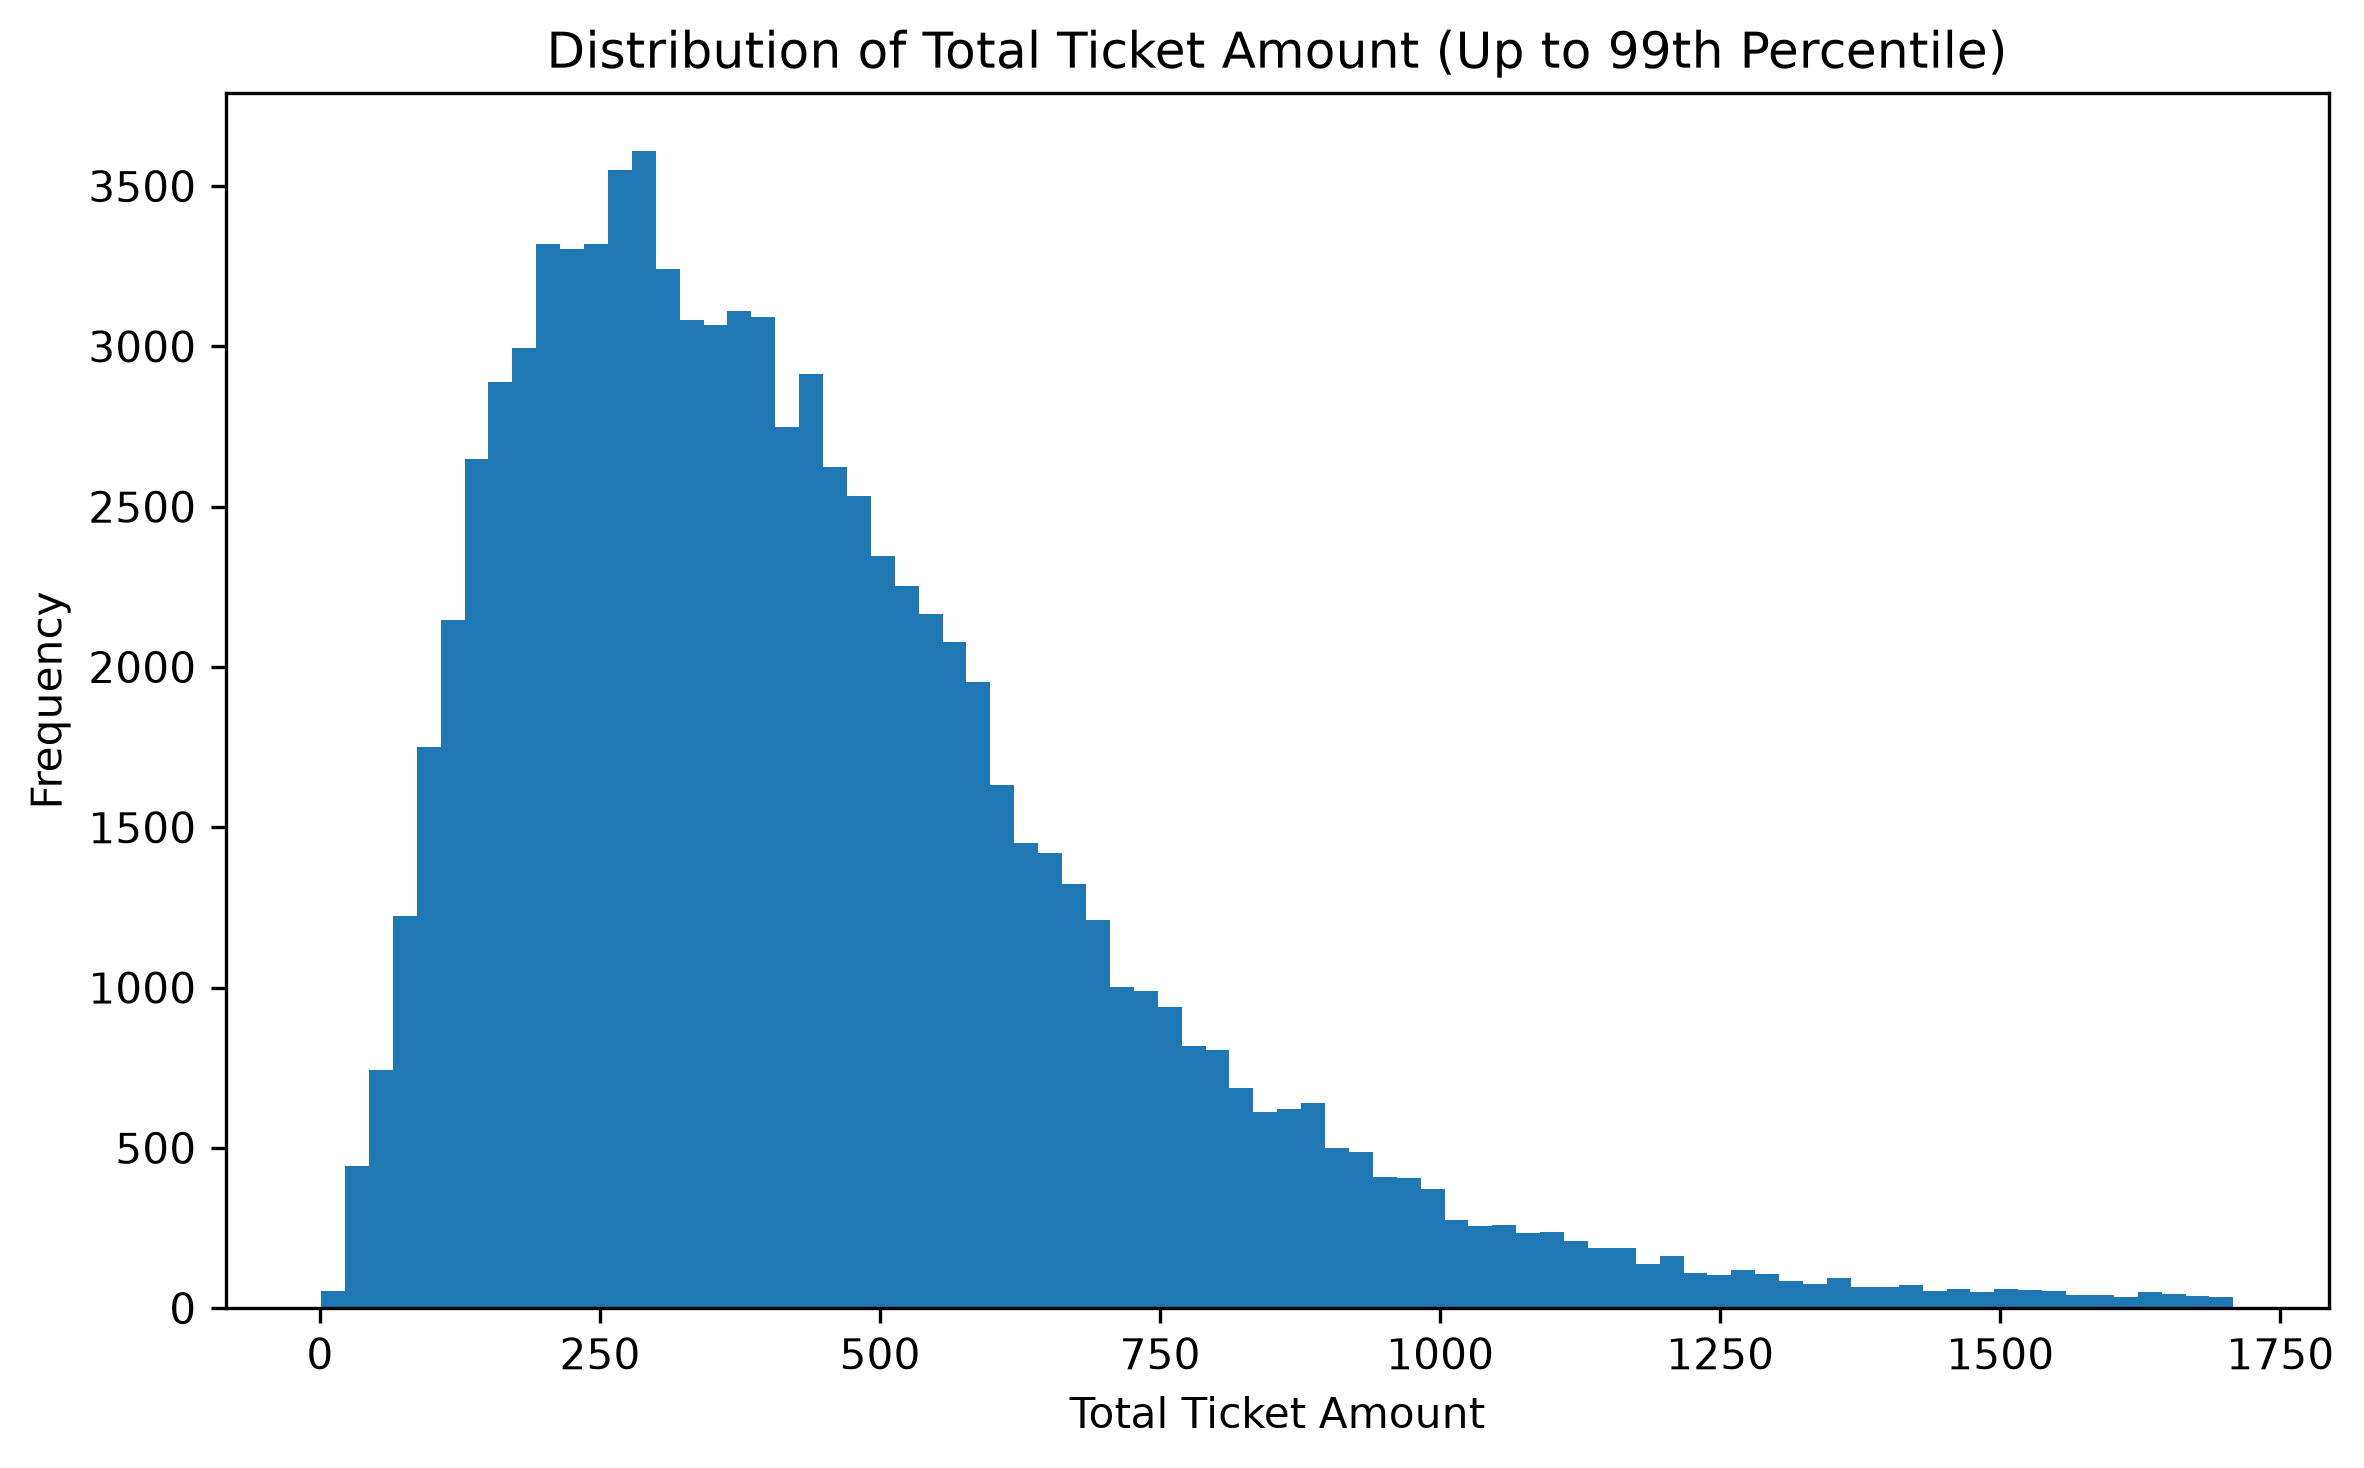
\includegraphics[width=0.78\textwidth]{../outputs/02_fare_distribution_p99.png}
\caption{Distribution of total ticket amount up to the 99th percentile}
\label{fig:fare-distribution}
\end{figure}

The figure confirms that fares are unimodal but clearly right-skewed rather than symmetric. No high-fare observations are removed at the exploratory stage. Their potential influence, and the implications of the skewed response distribution for linear-model assumptions, are assessed formally in the diagnostic stage.

\subsection{Distance and Itinerary Complexity}

\texttt{TotalDistance} also exhibits considerable variation. The median itinerary distance is 1,600 miles, compared with a mean of approximately 1,925 miles. Most itineraries are below 5,000 miles, although a small number extend substantially further.

The relationship between distance and fare is clearly positive. The Pearson correlation between \texttt{TotalDistance} and \texttt{TotalAmount} is

\[
r = 0.474.
\]

This indicates a moderate positive linear association.

\begin{figure}[H]
\centering
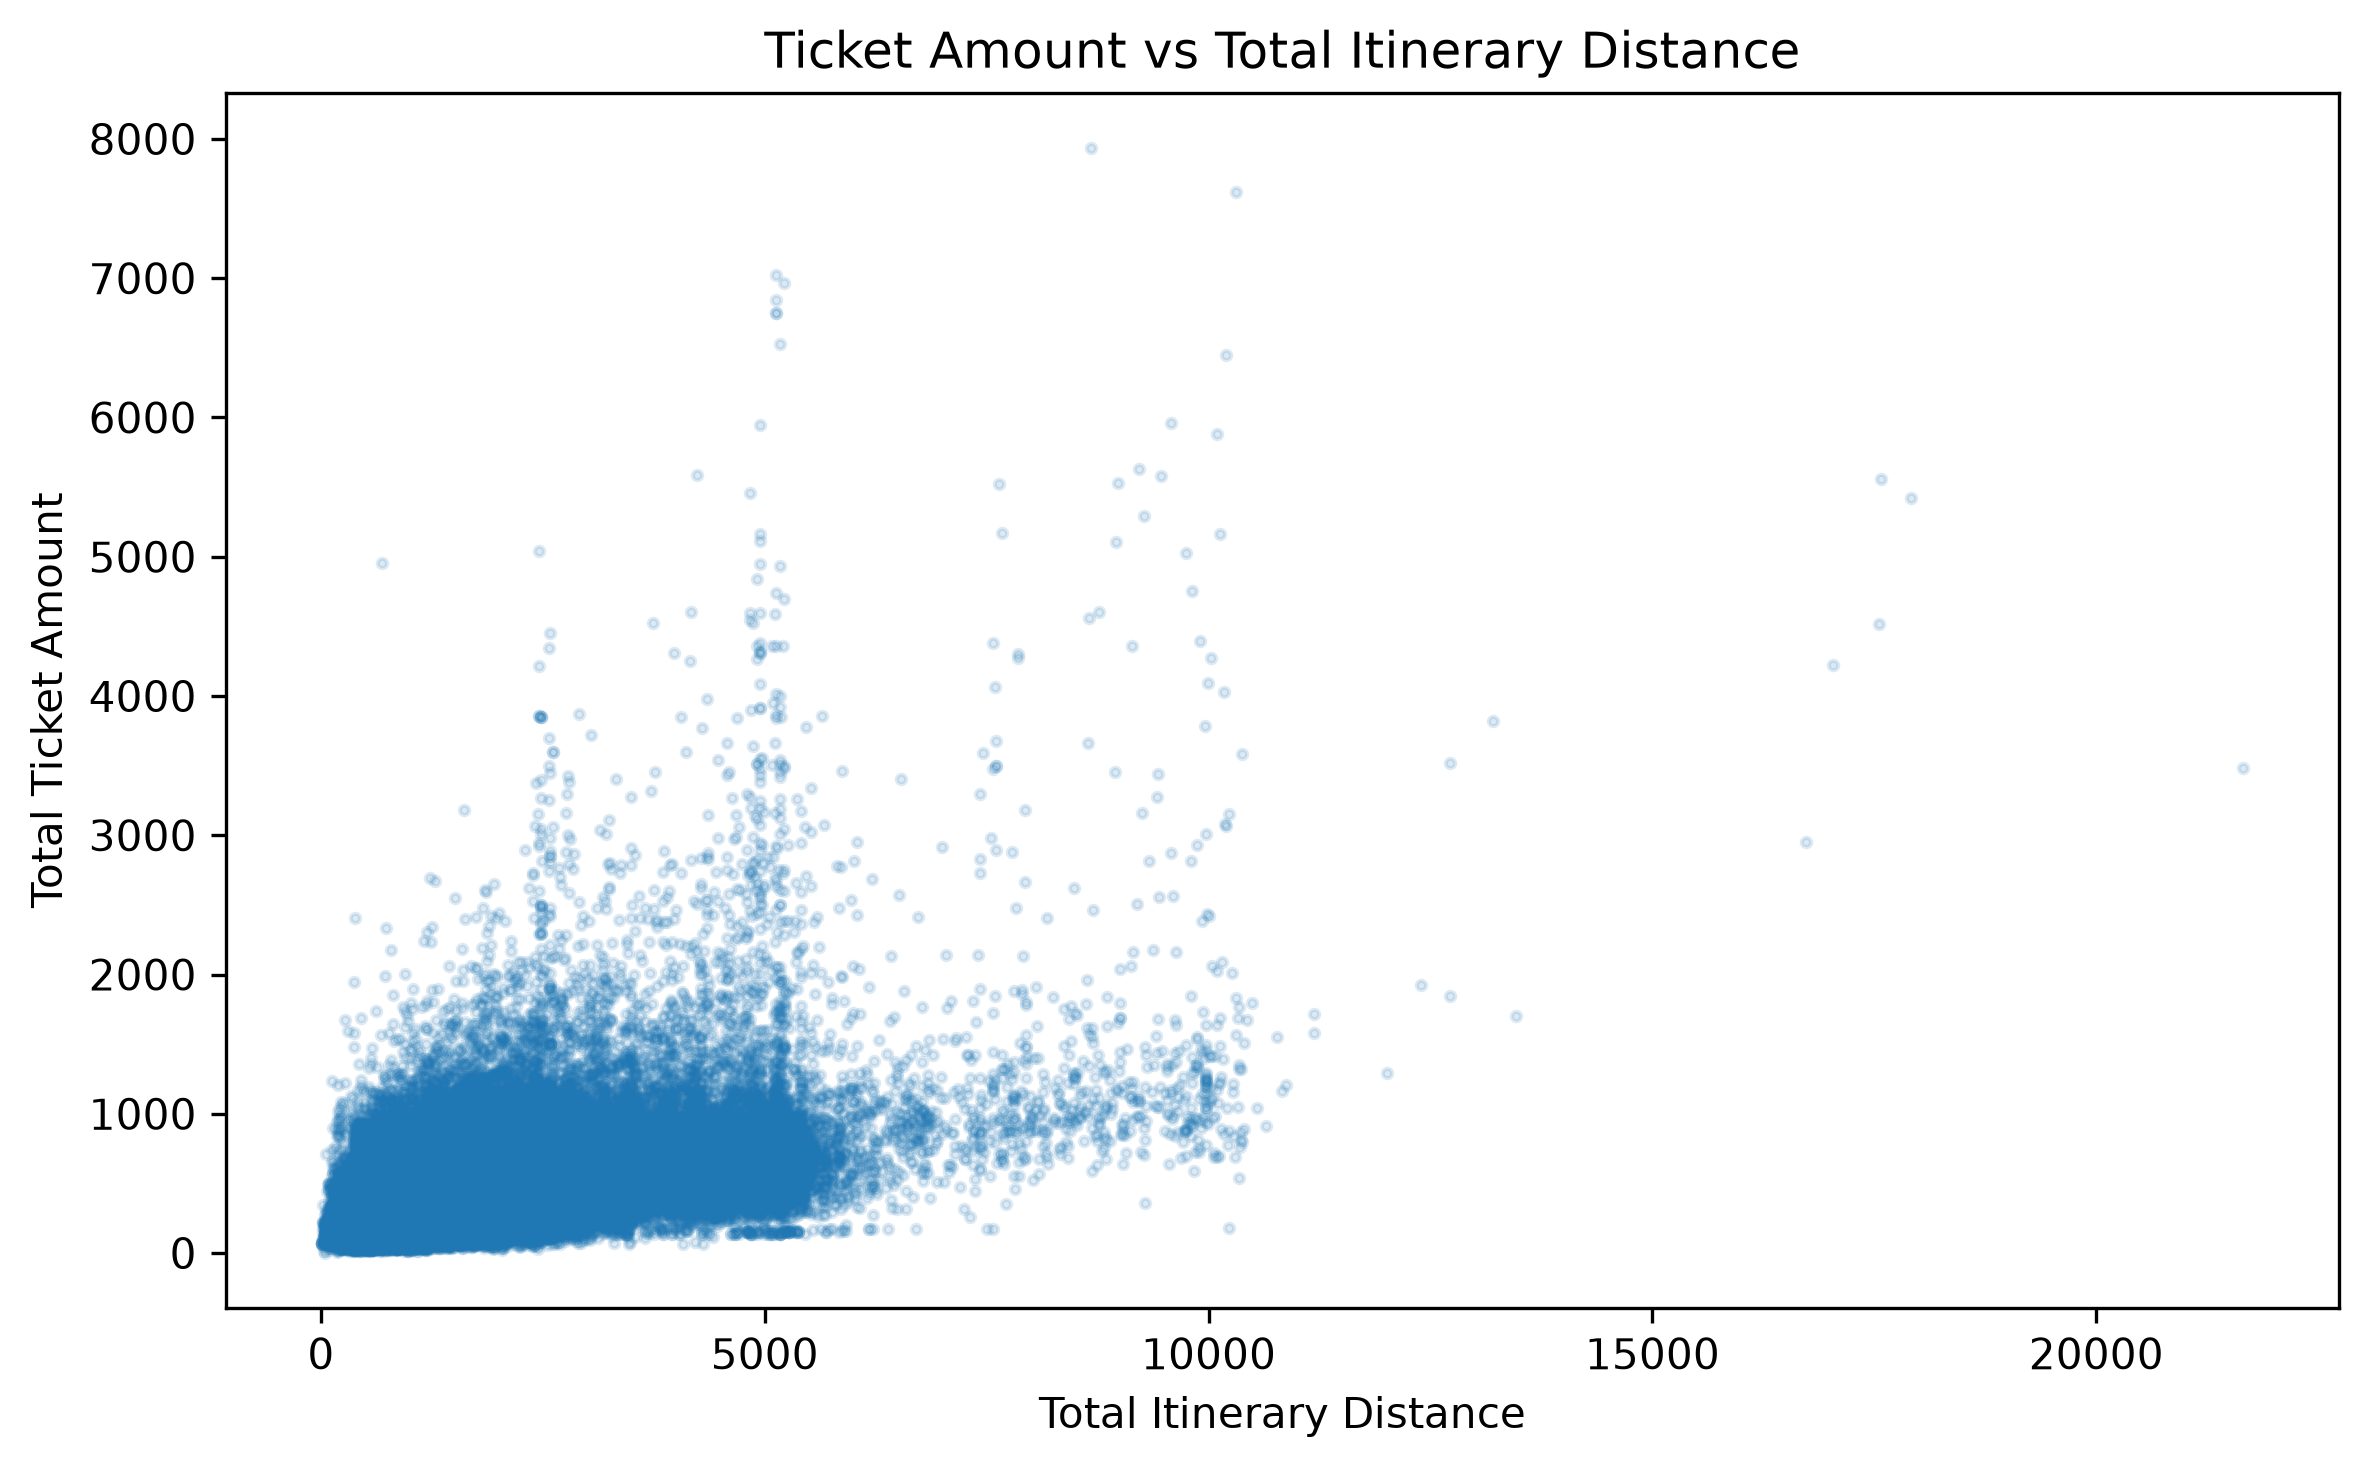
\includegraphics[width=0.78\textwidth]{../outputs/02_fare_vs_distance.png}
\caption{Total ticket amount versus total itinerary distance}
\label{fig:fare-distance}
\end{figure}

Figure~\ref{fig:fare-distance} shows that longer itineraries generally command higher ticket amounts, but also reveals substantial dispersion around the relationship. Tickets covering similar distances can have markedly different fares, indicating that distance alone is insufficient to explain observed price variation.

The number of ticket coupons provides a complementary measure of itinerary complexity. Coupon counts are concentrated at low values: 31.38\% of observations contain one coupon and 52.23\% contain two. Median fare generally increases with the number of coupons, rising from approximately \$242 for one-coupon itineraries to \$429 for two coupons, \$549 for three coupons, and \$626 for four coupons.

This pattern suggests that more complex itineraries tend to be associated with higher ticket amounts. However, very high coupon counts occur only rarely and are not interpreted as stable descriptive patterns.

\subsection{Categorical Fare Patterns}

The binary and low-cardinality categorical predictors also exhibit meaningful differences in unconditional fare levels. Table~\ref{tab:categorical-eda} reports the median fare and sample share for the principal categories.

\begin{table}[H]
\centering
\caption{Descriptive fare patterns across categorical predictors}
\label{tab:categorical-eda}
\begin{tabular}{llrr}
\toprule
\textbf{Variable} & \textbf{Category} & \textbf{Median fare (\$)} & \textbf{Sample share} \\
\midrule
\texttt{RoundTrip} & 0 & 268.40 & 45.04\% \\
\texttt{RoundTrip} & 1 & 510.38 & 54.96\% \\
\addlinespace
\texttt{OnLine} & 0 & 549.76 & 13.07\% \\
\texttt{OnLine} & 1 & 365.80 & 86.93\% \\
\addlinespace
\texttt{PurchaseWindowGroup} & 21AP & 425.86 & 46.11\% \\
\texttt{PurchaseWindowGroup} & 2290 & 355.50 & 42.75\% \\
\texttt{PurchaseWindowGroup} & 91UP & 386.40 & 11.13\% \\
\addlinespace
\texttt{ItinGeoType} & 1 & 450.32 & 7.87\% \\
\texttt{ItinGeoType} & 2 & 384.81 & 92.13\% \\
\bottomrule
\end{tabular}
\end{table}

Round-trip tickets have substantially higher unconditional fares than one-way tickets, with median fares of \$510.38 and \$268.40 respectively. This difference should not be interpreted as a round-trip premium, because round-trip itineraries may also differ systematically in distance and number of coupons.

The \texttt{OnLine} indicator also separates tickets with noticeably different fare distributions. Although \texttt{OnLine = 1} represents 86.93\% of observations, the smaller \texttt{OnLine = 0} group still contains more than 11,000 tickets and has a considerably higher median fare.

Purchase-window categories display meaningful but non-monotonic differences in median fare. The category labels are treated as categorical codes rather than assigned an ordinal numerical interpretation.

Finally, \texttt{ItinGeoType = 1} is associated with a higher unconditional median fare than \texttt{ItinGeoType = 2}. Both categories contain sufficient observations for subsequent regression modelling despite the imbalance in their frequencies.

These comparisons are deliberately descriptive. The observed differences may reflect other correlated ticket characteristics and therefore require a multiple-regression framework before conditional effects can be interpreted.

\subsection{Carrier and Geographic Variation}

Carrier identity is associated with particularly large differences in unconditional fare levels. The four largest reporting carriers---\texttt{AA}, \texttt{WN}, \texttt{DL}, and \texttt{UA}---together account for approximately three quarters of the analysis sample, while a long tail of smaller carriers contributes relatively few observations.

For visual clarity, Figure~\ref{fig:carrier-fares} displays carriers with at least 100 observations. The threshold is used only for presentation; no observations are removed from the regression dataset at this stage.

\begin{figure}[H]
\centering
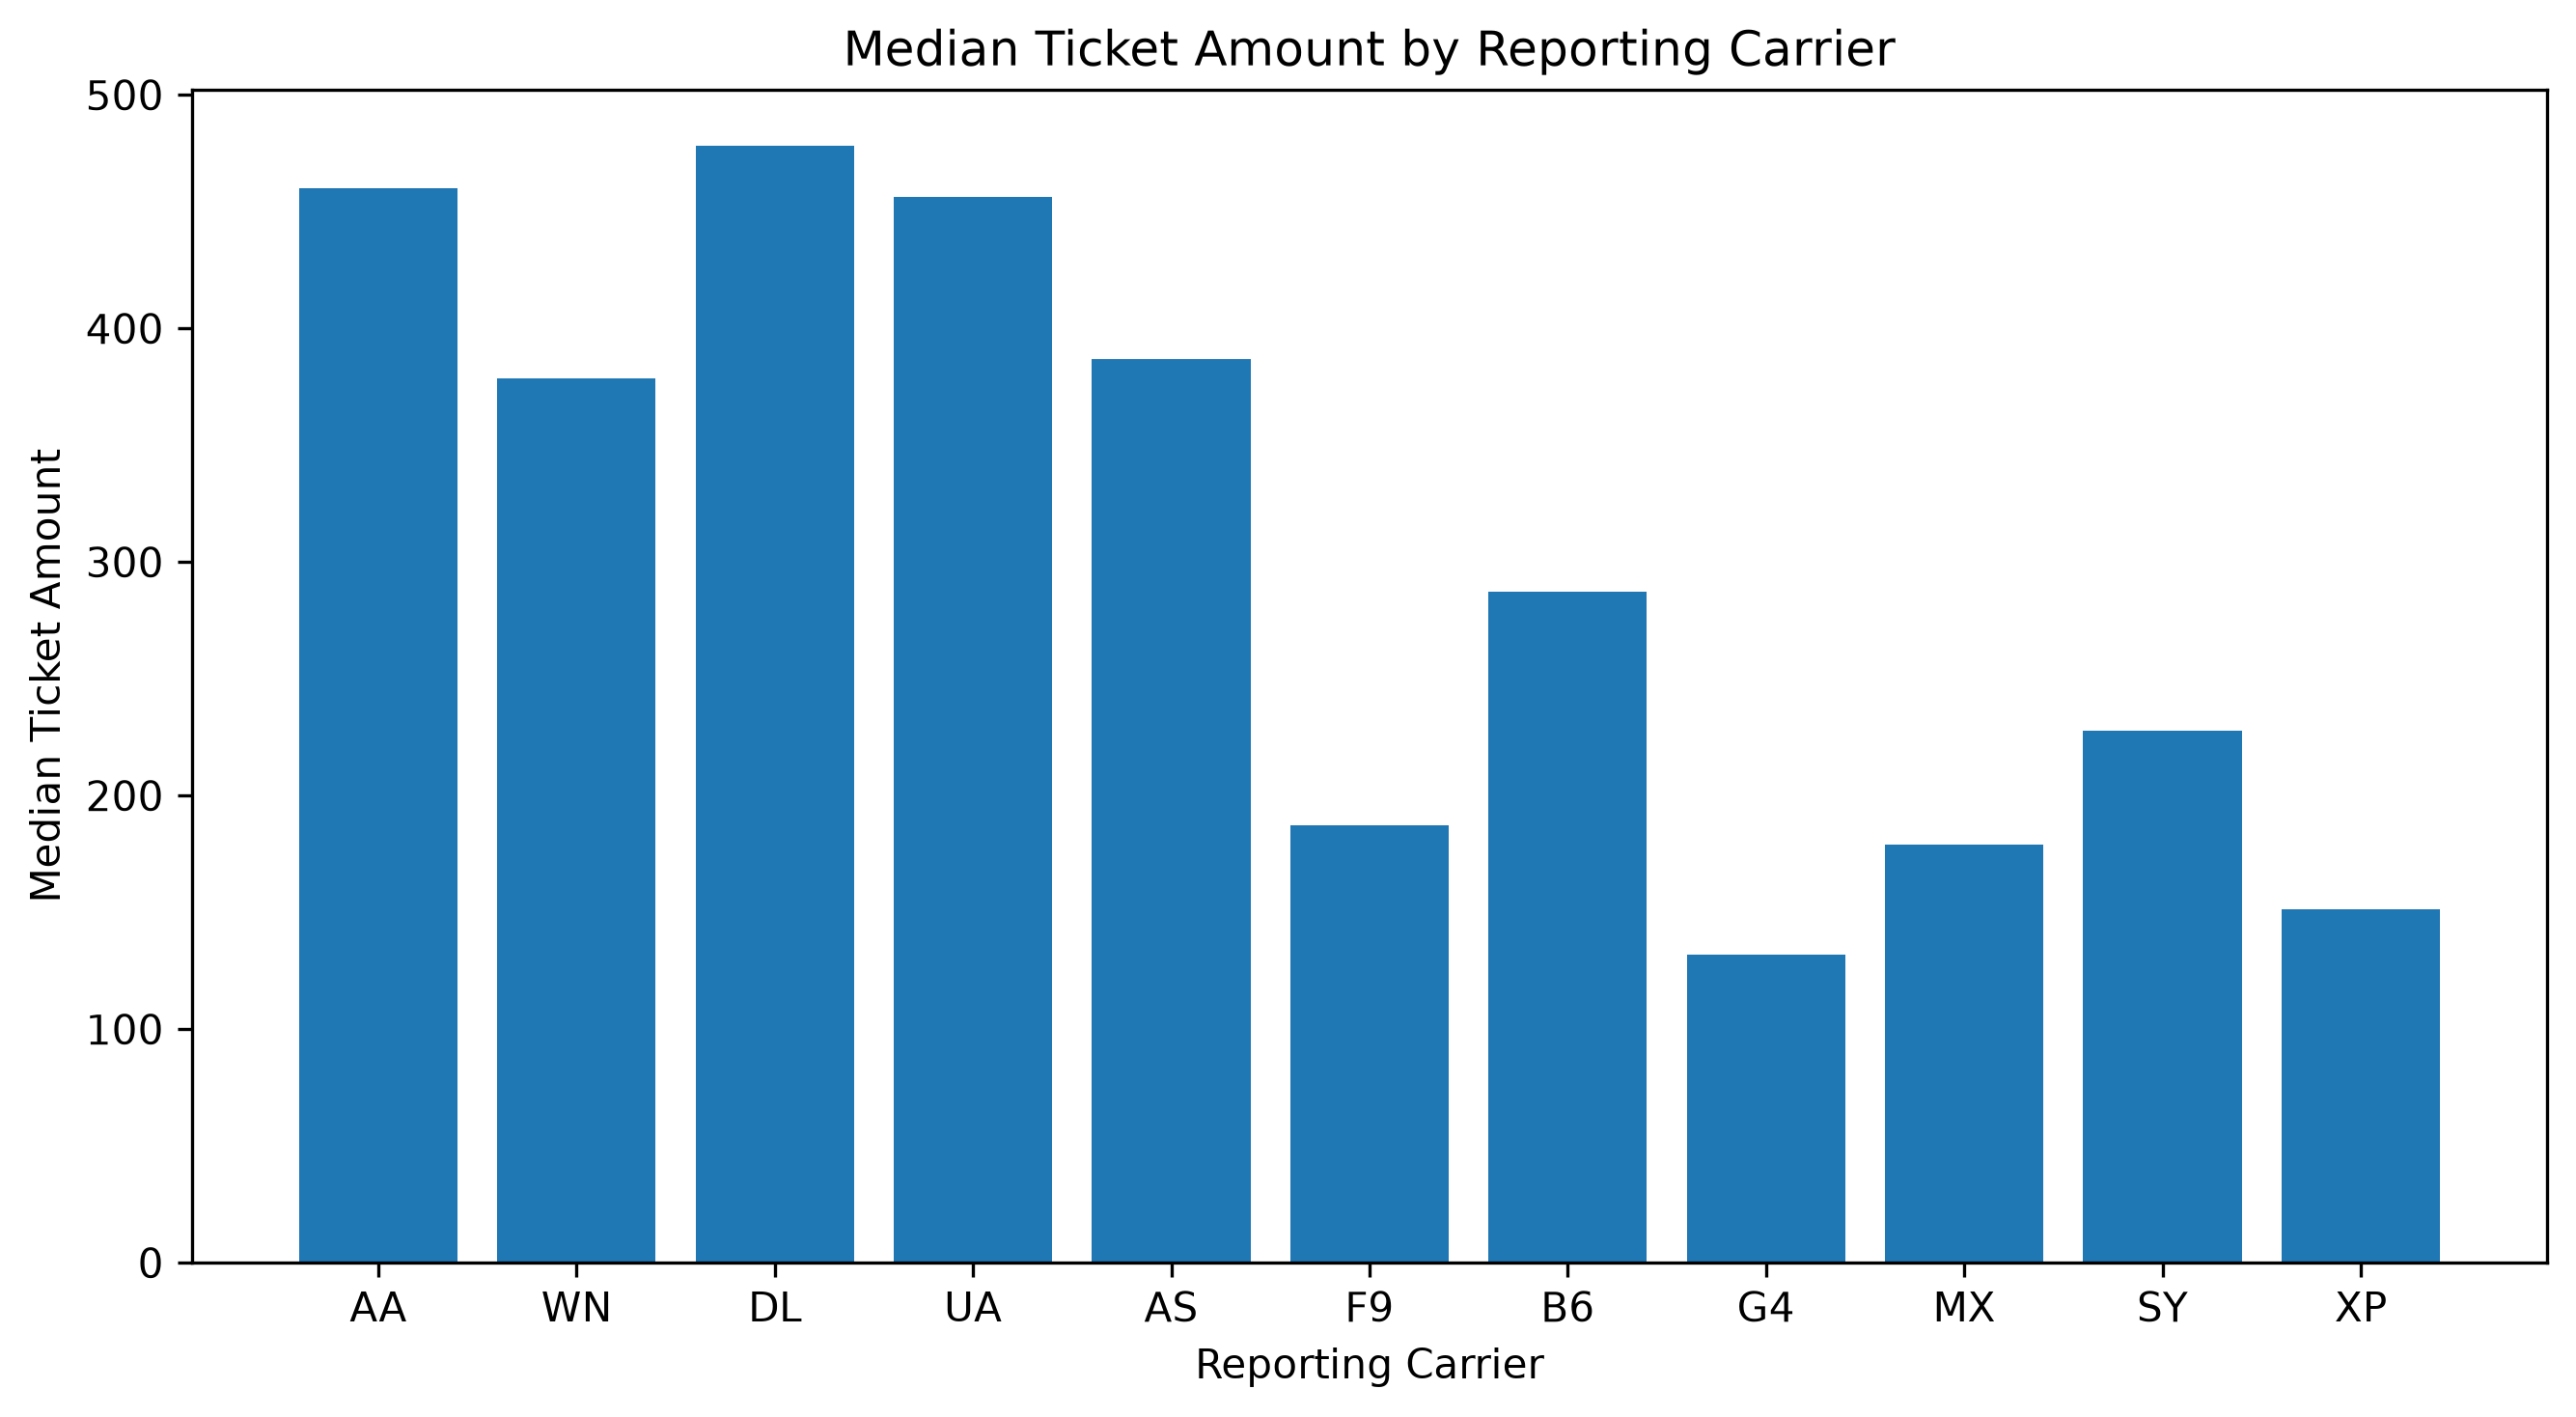
\includegraphics[width=0.82\textwidth]{../outputs/02_carrier_median_fare.png}
\caption{Median ticket amount by reporting carrier for carriers with at least 100 observations}
\label{fig:carrier-fares}
\end{figure}

Among the well-represented carriers, median fares range widely. \texttt{DL}, \texttt{AA}, and \texttt{UA} have median fares of approximately \$478, \$460, and \$456 respectively, whereas carriers such as \texttt{F9}, \texttt{G4}, \texttt{MX}, and \texttt{XP} display considerably lower unconditional median fares.

These differences suggest that carrier identity contains potentially important explanatory information. However, raw carrier comparisons may also reflect differences in route length, network structure, itinerary composition, geography, or purchase characteristics and therefore should not be interpreted as carrier effects in isolation.

Origin-state fare levels also vary substantially. Figure~\ref{fig:state-fares} displays states or territories with at least 500 observations for visual clarity.

\begin{figure}[H]
\centering
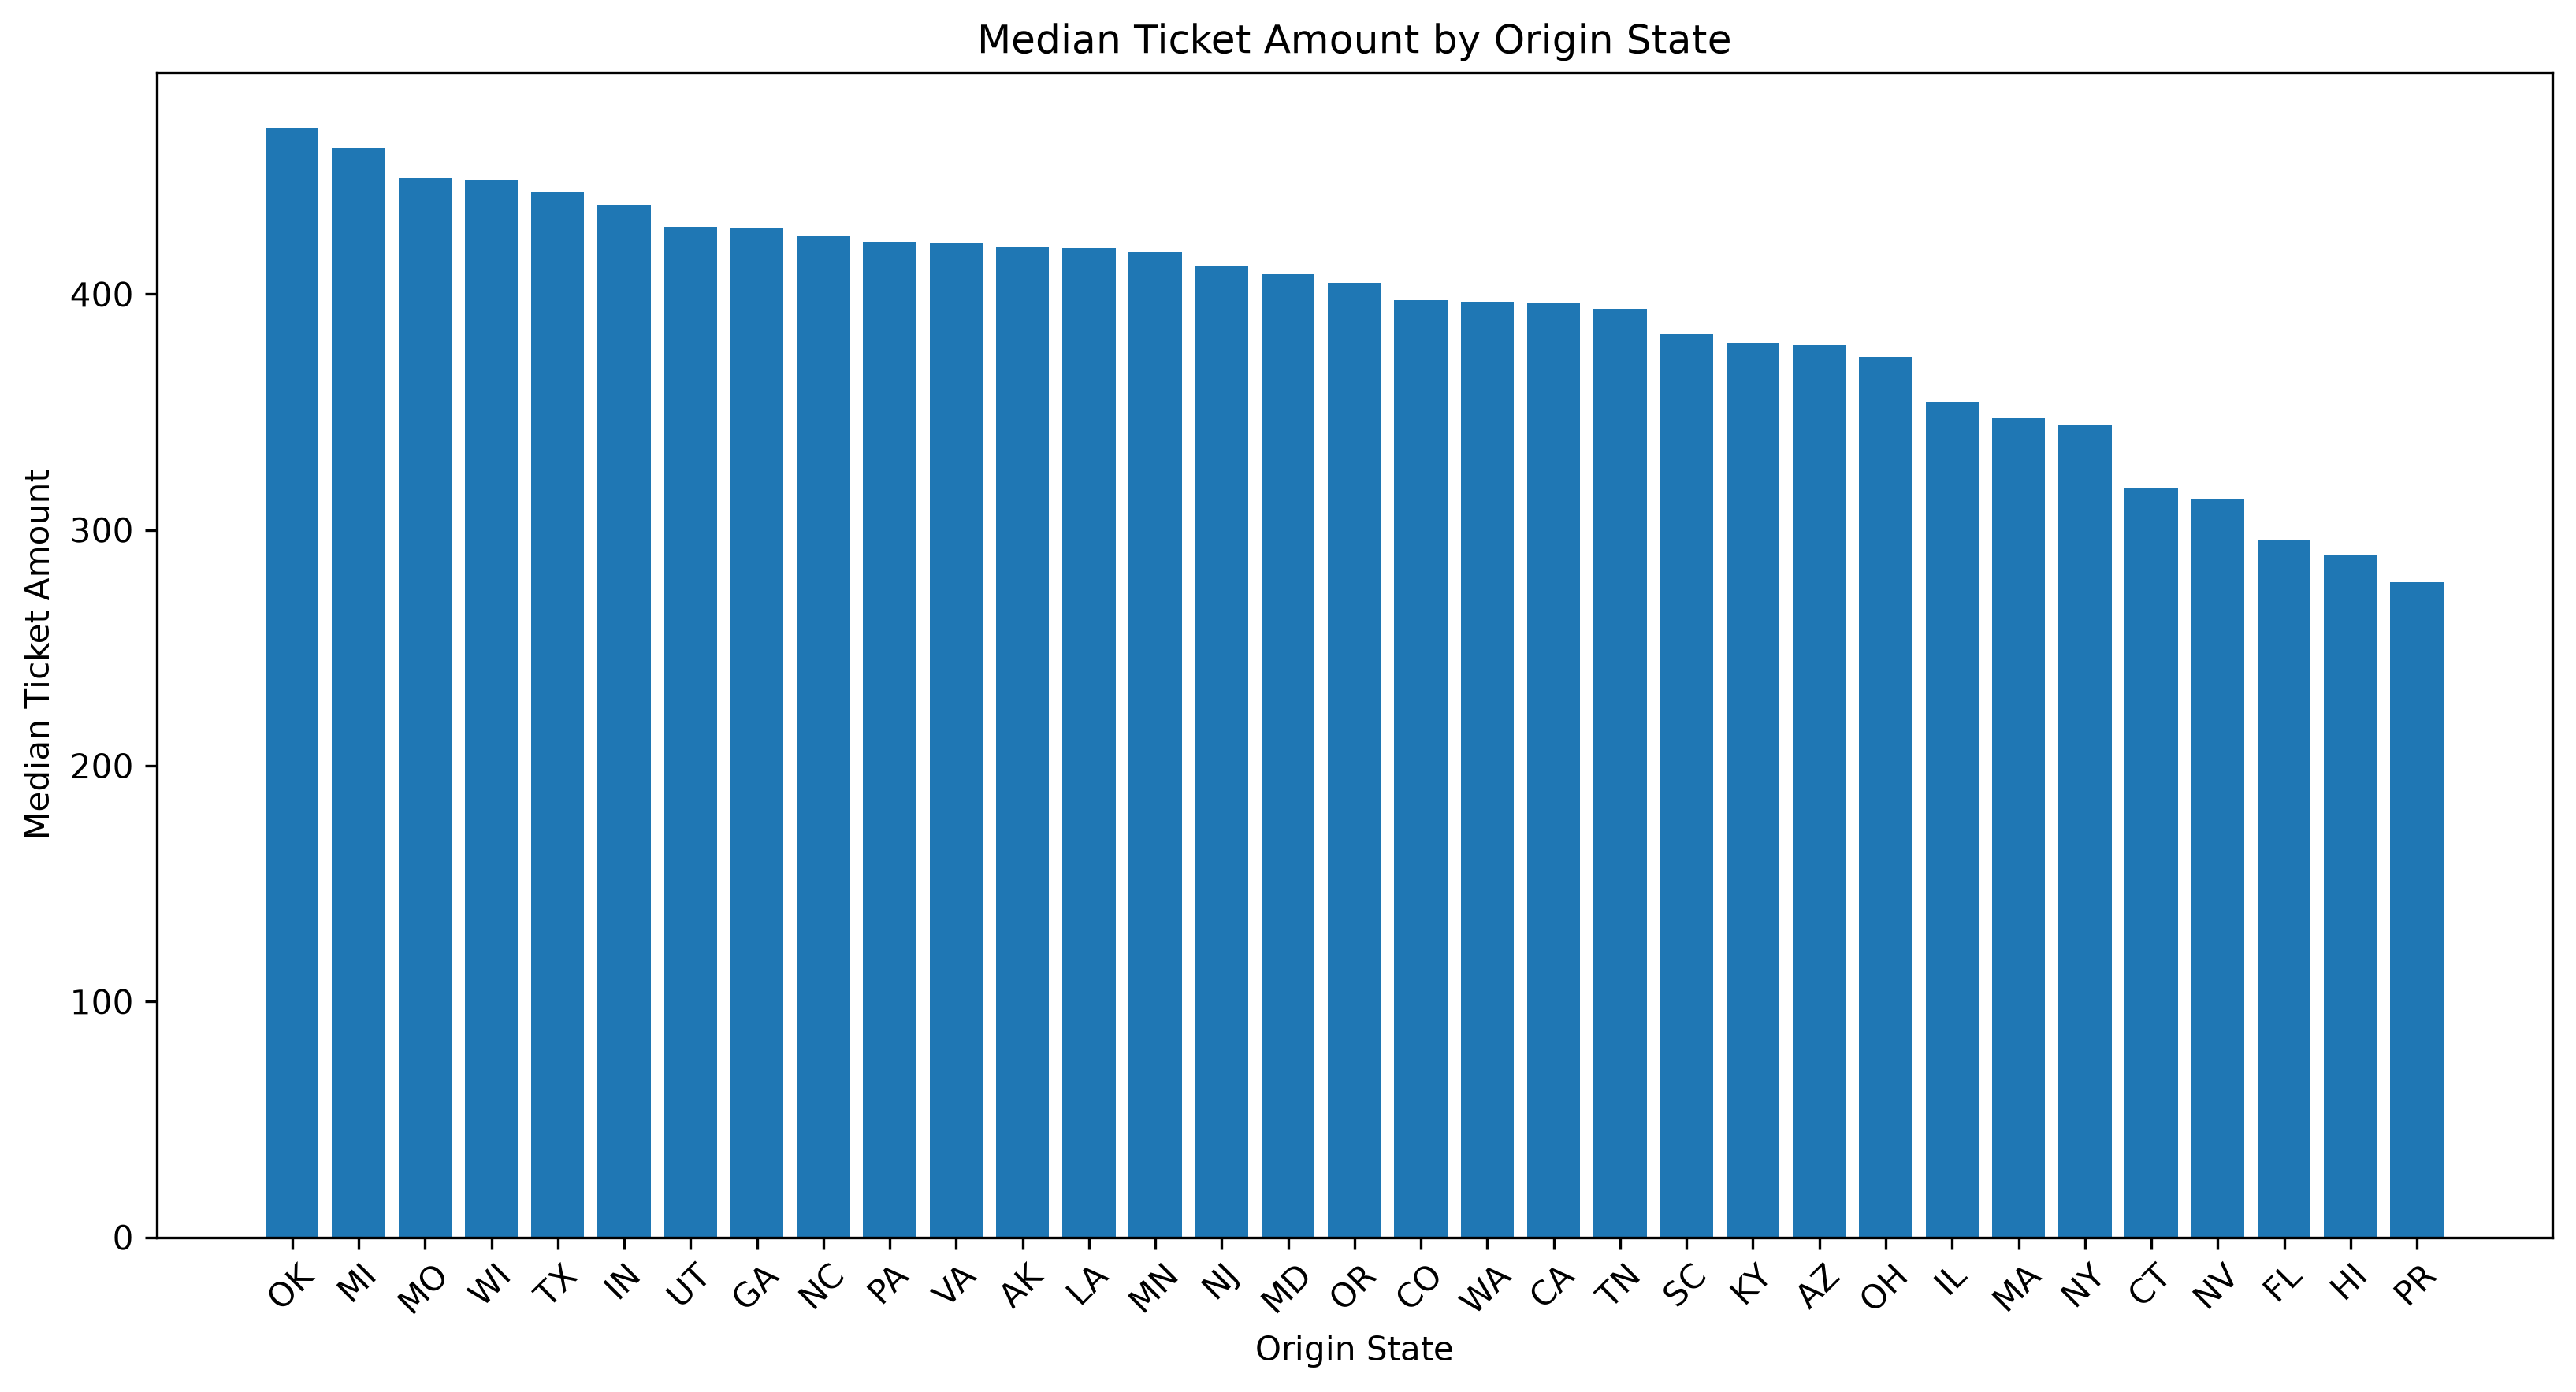
\includegraphics[width=0.88\textwidth]{../outputs/02_state_median_fare.png}
\caption{Median ticket amount by origin state for states or territories with at least 500 observations}
\label{fig:state-fares}
\end{figure}

Among the displayed states, median fares range from roughly the high-\$200s to the high-\$400s. Oklahoma, Michigan, Missouri, and Wisconsin are among the higher-median-fare origin states, whereas Florida, Puerto Rico, Hawaii, and Nevada are among the lower-fare groups.

As with carrier comparisons, these geographic differences are unconditional. They may partly reflect differences in route length, carrier mix, itinerary structure, or other travel characteristics. The results nevertheless support retaining origin geography as a candidate explanatory dimension.

\subsection{Relationships Among Candidate Predictors}

Exploratory analysis also considers whether the candidate predictors appear so strongly related that they provide effectively duplicate information.

For the principal numerical variables, the sample correlation matrix is:

\begin{table}[H]
\centering
\caption{Correlations among fare, distance, and itinerary complexity}
\label{tab:eda-correlation}
\begin{tabular}{lrrr}
\toprule
& \textbf{TotalAmount} & \textbf{TotalDistance} & \textbf{Coupons} \\
\midrule
\texttt{TotalAmount} & 1.000 & 0.474 & 0.407 \\
\texttt{TotalDistance} & 0.474 & 1.000 & 0.536 \\
\texttt{Coupons} & 0.407 & 0.536 & 1.000 \\
\bottomrule
\end{tabular}
\end{table}

\texttt{TotalDistance} and \texttt{Coupons} have a moderate positive correlation of 0.536. This is economically intuitive because itineraries containing more ticketed segments also tend to cover greater total distances. The relationship is not sufficiently strong, however, to suggest that the two variables represent the same information: distance measures the extent of travel, whereas coupons capture itinerary complexity.

A similar structural relationship appears between \texttt{RoundTrip} and \texttt{Coupons}. Among one-way itineraries, 69.67\% contain one coupon and 28.49\% contain two. In contrast, 71.69\% of round-trip itineraries contain two coupons and a further 21.39\% contain four.

The overlap is expected from the structure of airline itineraries, but the two variables remain conceptually distinct. \texttt{RoundTrip} identifies whether the itinerary returns to its origin, whereas \texttt{Coupons} measures the number of ticketed segments.

Formal assessment of multicollinearity is therefore deferred to the regression stage rather than inferred from these descriptive associations alone.

\subsection{Exploratory Findings}

The exploratory evidence supports carrying all eight pre-screened predictor blocks into the initial broad regression model.

Several patterns are particularly relevant for the subsequent modelling:

\begin{itemize}
    \item ticket fares are positively skewed and contain a long upper tail;
    \item itinerary distance has a moderate positive relationship with fare but leaves substantial unexplained dispersion;
    \item greater itinerary complexity is generally associated with higher fares;
    \item round-trip status, carrier structure, purchase timing, and itinerary geography all correspond to meaningful differences in unconditional fare distributions;
    \item carrier and origin-state fare levels vary materially across groups; and
    \item some candidate predictors are related to one another, particularly distance, coupons, and round-trip status, but none appears descriptively redundant.
\end{itemize}

Accordingly, no candidate predictor is removed on the basis of exploratory analysis alone. The eight predictor blocks are carried forward to the initial multiple-regression model, where their joint contribution and multicollinearity are assessed formally.

% ============================================================
% SECTION 4 - INITIAL BROAD REGRESSION MODEL
% ============================================================

\section{Initial Broad Regression Model}

\noindent\textit{Code reference: Notebook 03 (\texttt{03\_initial\_broad\_model.ipynb}).}

\subsection{Model-Building and Validation Samples}

Before any regression model is estimated, the prepared sample is divided randomly into equal model-building and validation samples using a fixed random seed of 42.

\begin{table}[H]
\centering
\caption{Model-building and validation sample split}
\label{tab:sample-split}
\begin{tabular}{lrr}
\toprule
\textbf{Sample} & \textbf{Observations} & \textbf{Share} \\
\midrule
Full prepared sample & 90,086 & 100.0\% \\
Model-building sample & 45,043 & 50.0\% \\
Validation sample & 45,043 & 50.0\% \\
\bottomrule
\end{tabular}
\end{table}

The model-building sample is used for the initial broad model, subsequent variable reduction, diagnostic assessment, and model refinement. The validation sample is held aside at this stage and is not used to influence model specification or refinement decisions.

This separation provides an independent sample for assessing out-of-sample performance after the candidate models have been finalised.

\subsection{Categorical Grouping and Reference Categories}

Several categorical predictors contain low-frequency levels. To avoid estimating coefficients from very small groups, categories with fewer than 100 observations in the model-building sample are consolidated into an \texttt{Other} category.

Importantly, the grouping rules are determined using the model-building sample only and then applied unchanged to the validation sample. This prevents information from the validation sample from influencing model construction.

After grouping:

\begin{itemize}
    \item \texttt{RpCarrier\_Model} contains 12 modelling categories, including \texttt{Other};
    \item \texttt{OriginState\_Model} contains 43 modelling categories, including \texttt{Other}.
\end{itemize}

The reference categories are selected as follows:

\begin{itemize}
    \item \texttt{RoundTrip = 0};
    \item \texttt{OnLine = 1};
    \item \texttt{PurchaseWindowGroup = 21AP};
    \item \texttt{RpCarrier\_Model = AA};
    \item \texttt{ItinGeoType = 2};
    \item \texttt{OriginState\_Model = CA}.
\end{itemize}

Categorical coefficients are therefore interpreted relative to these reference groups, holding the remaining predictors constant.

\subsection{Broad Model Specification}

The initial regression deliberately includes all eight candidate predictor blocks identified during data preparation and exploratory analysis:

\[
\begin{aligned}
\text{TotalAmount}_i
={}&
\beta_0
+\beta_1 \text{TotalDistance}_i
+\beta_2 \text{Coupons}_i \\
&+\text{RoundTrip effects}
+\text{OnLine effects}
+\text{PurchaseWindowGroup effects} \\
&+\text{Carrier effects}
+\text{Itinerary geography effects}
+\text{Origin-state effects}
+\varepsilon_i.
\end{aligned}
\]

The model is intentionally broad. No predictor is removed at this stage on the basis of an individual coefficient or p-value.

The purpose of this specification is to establish a common baseline from which the contribution of individual predictor blocks can later be evaluated.

\subsection{Overall Model Fit}

The broad OLS model is estimated using the 45,043-observation model-building sample.

\begin{table}[H]
\centering
\caption{Initial broad-model summary}
\label{tab:broad-model-summary}
\begin{tabular}{lr}
\toprule
\textbf{Metric} & \textbf{Value} \\
\midrule
Observations & 45,043 \\
Model degrees of freedom & 60 \\
Residual degrees of freedom & 44,982 \\
$R^2$ & 0.385 \\
$F$-statistic & 470.2 \\
Overall $F$-test p-value & $<0.001$ \\
\bottomrule
\end{tabular}
\end{table}

The model is highly statistically significant overall. An \(R^2\) of 0.385 indicates that the eight predictor blocks jointly explain approximately 38.5\% of the observed cross-sectional variation in total ticket amount within the model-building sample.

This represents meaningful explanatory power for a ticket-level cross-sectional model, although a substantial proportion of fare variation remains attributable to characteristics not captured by the available predictors.

\subsection{Initial Coefficient Patterns}

Table~\ref{tab:broad-key-coefficients} reports selected coefficients from the broad model. The table focuses on the principal continuous, binary, and low-cardinality predictors; the complete set of carrier and origin-state coefficients is retained in the model output rather than reproduced in the main text.

\begin{table}[H]
\centering
\caption{Selected coefficients from the initial broad OLS model}
\label{tab:broad-key-coefficients}
\begin{tabular}{lrrr}
\toprule
\textbf{Predictor} & \textbf{Coefficient} & \textbf{Std. error} & \textbf{p-value} \\
\midrule
\texttt{TotalDistance} & 0.094 & 0.001 & $<0.001$ \\
\texttt{Coupons} & 3.873 & 2.309 & 0.093 \\
\texttt{RoundTrip = 1} & 140.997 & 3.577 & $<0.001$ \\
\texttt{OnLine = 0} & 64.301 & 4.822 & $<0.001$ \\
\texttt{PurchaseWindowGroup = 2290} & -128.766 & 2.812 & $<0.001$ \\
\texttt{PurchaseWindowGroup = 91UP} & -137.351 & 4.475 & $<0.001$ \\
\texttt{ItinGeoType = 1} & 47.129 & 6.993 & $<0.001$ \\
\bottomrule
\end{tabular}
\end{table}

Several conditional relationships are already apparent.

\texttt{TotalDistance} is positively associated with ticket amount: holding the other predictors fixed, the fitted fare increases by approximately \$0.094 for each additional mile in the level-fare specification.

Round-trip itineraries are associated with fares approximately \$141 higher than otherwise comparable one-way itineraries. Similarly, \texttt{OnLine = 0} is associated with fares approximately \$64 higher than the \texttt{OnLine = 1} reference group.

Both non-reference purchase-window categories are associated with substantially lower fitted fares than \texttt{21AP}, while \texttt{ItinGeoType = 1} is associated with fitted fares approximately \$47 higher than \texttt{ItinGeoType = 2}.

Carrier effects also vary materially relative to American Airlines, and several origin-state coefficients differ significantly from California. However, many individual state coefficients are not statistically significant, so isolated dummy-variable p-values are not used to remove entire categorical predictor blocks.

The notable exception among the principal predictors is \texttt{Coupons}. Its estimated coefficient is positive but not statistically significant at the 5\% level:

\[
\hat{\beta}_{\text{Coupons}} = 3.873,
\qquad
t = 1.678,
\qquad
p = 0.093.
\]

This provides a natural candidate for later variable-reduction analysis, but it is not removed at this stage.

\subsection{Multicollinearity Assessment}

Because several predictors describe related aspects of itinerary structure, multicollinearity is assessed before proceeding to formal variable selection.

The correlation between the two numerical predictors is:

\[
r(\text{TotalDistance},\text{Coupons}) = 0.539.
\]

This indicates a moderate positive relationship but is not sufficiently large, by itself, to suggest severe linear dependence.

Variance inflation factors provide a more direct assessment of multicollinearity in the full model.

\begin{table}[H]
\centering
\caption{Multicollinearity summary for the initial broad model}
\label{tab:multicollinearity-summary}
\begin{tabular}{lr}
\toprule
\textbf{Measure} & \textbf{Value} \\
\midrule
Correlation: \texttt{TotalDistance} vs \texttt{Coupons} & 0.539 \\
Maximum VIF excluding intercept & 3.01 \\
Mean VIF excluding intercept & 1.31 \\
VIF: \texttt{Coupons} & 3.01 \\
VIF: \texttt{ItinGeoType} & 2.11 \\
VIF: \texttt{TotalDistance} & 1.94 \\
\bottomrule
\end{tabular}
\end{table}

All VIFs are well below the threshold of 10 used in the course material. The overall regression is also highly significant, while many individual coefficients remain statistically significant.

There is therefore no evidence that severe multicollinearity is materially distorting the broad-model estimates. No predictor is removed on multicollinearity grounds.

\subsection{Broad-Model Assessment}

The initial broad model establishes several points before formal variable selection begins.

First, the eight predictor blocks jointly provide a statistically significant explanation of cross-sectional fare variation.

Second, the principal itinerary, purchase, carrier, and geographic variables exhibit meaningful conditional associations with total ticket amount.

Third, multicollinearity does not appear to be a material concern.

The main unresolved issue is the incremental contribution of \texttt{Coupons}. Although its coefficient is positive, it is not statistically significant at the 5\% level in the broad level-fare model.

Accordingly, no variable is removed at this stage. Formal variable reduction and comparison of nearby subset models are conducted in the next stage.

% ============================================================
% SECTION 5 - VARIABLE REDUCTION AND CANDIDATE MODEL SELECTION
% ============================================================

\section{Variable Reduction and Candidate Model Selection}

\noindent\textit{Code reference: Notebook 04 (\texttt{04\_variable\_reduction.ipynb}).}

The initial broad model contains eight conceptual predictor blocks. Variable reduction is conducted on the model-building sample only; the reserved validation sample remains unused throughout this stage.

Categorical predictors are treated as complete blocks. For example, removing \texttt{OriginState\_Model} means removing all associated state dummy variables together rather than selecting individual dummy coefficients separately.

\subsection{Backward Selection}

Backward selection is first used to identify an approximate preferred model size. Starting from the full eight-block model, each predictor block is removed in turn and the resulting reduced model is compared with the current model using a partial \(F\)-test.

At the first step, \texttt{Coupons} has the largest removal p-value:

\[
F = 2.815,
\qquad
p = 0.0934.
\]

At the 5\% significance level, there is insufficient evidence that \texttt{Coupons} provides additional explanatory value once the other seven predictor blocks are included. It is therefore removed by the automatic procedure.

After re-estimating the model without \texttt{Coupons}, all seven remaining predictor blocks have statistically significant partial \(F\)-tests. The backward-selection procedure therefore terminates with the following seven-block specification:

\begin{itemize}
    \item \texttt{TotalDistance};
    \item \texttt{RoundTrip};
    \item \texttt{OnLine};
    \item \texttt{PurchaseWindowGroup};
    \item \texttt{RpCarrier\_Model};
    \item \texttt{ItinGeoType};
    \item \texttt{OriginState\_Model}.
\end{itemize}

The backward-selected model is not accepted automatically as the final specification. Instead, the result is treated as evidence that approximately seven predictor blocks may provide an appropriate balance between explanatory performance and model complexity.

\subsection{Nearby-Subset Search}

To assess whether the backward-selected model is genuinely preferable, all specifications containing six, seven, or eight predictor blocks are estimated.

With eight available predictor blocks, the search contains

\[
\binom{8}{6}+\binom{8}{7}+\binom{8}{8}
=
28+8+1
=
37
\]

candidate models.

The models are compared using six criteria:

\begin{itemize}
    \item \(R^2\), where larger values indicate greater in-sample explanatory fit;
    \item adjusted \(R^2\), which penalises additional estimated parameters;
    \item Mallows' \(C_p\), where relatively small values close to the number of estimated parameters \(p\) are preferred;
    \item AIC, where smaller values are preferred;
    \item BIC/SBC, which applies a stronger complexity penalty than AIC; and
    \item PRESS, where smaller values indicate better leave-one-out predictive performance.
\end{itemize}

Because ordinary \(R^2\) cannot decrease when predictors are added, it is not used in isolation to select the preferred model.

\subsection{Comparison of Leading Specifications}

The model-selection criteria do not identify a single specification that dominates on every dimension. Table~\ref{tab:model-selection-comparison} compares the three most relevant specifications.

\begin{table}[H]
\centering
\caption{Comparison of leading candidate specifications}
\label{tab:model-selection-comparison}
\small
\begin{tabular}{lrrrrrr}
\toprule
\textbf{Specification} & \textbf{Parameters} & \(\mathbf{R^2}\) & \(\mathbf{Adj.\ R^2}\) & \(\mathbf{C_p}\) & \textbf{AIC} & \textbf{PRESS} \\
\midrule
Full 8-block & 61 & 0.385439 & 0.384619 & 61.00 & 634313.98 & \(3.443909\times10^9\) \\
7-block, no Coupons & 60 & 0.385401 & 0.384595 & 61.82 & 634314.80 & \(3.443877\times10^9\) \\
BIC-selected 6-block & 18 & 0.379576 & 0.379341 & 404.17 & 634655.70 & \(3.470603\times10^9\) \\
\bottomrule
\end{tabular}
\end{table}

The full eight-block model produces the highest \(R^2\) and adjusted \(R^2\), the lowest AIC, and a Mallows' \(C_p\) equal to the number of estimated parameters. The equality \(C_p=p=61\) is expected because the full model provides the reference estimate of the error variance used in the \(C_p\) calculation.

The backward-selected seven-block model performs almost identically. Its adjusted \(R^2\) is 0.384595 compared with 0.384619 for the full model, while its AIC differs by less than one point. Its Mallows' \(C_p\) is also close to its parameter count:

\[
C_p = 61.82,
\qquad
p = 60.
\]

The seven-block specification also produces the lowest PRESS among the 37 nearby candidate models, although the difference from the full model is extremely small. Thus, removing \texttt{Coupons} produces almost no loss in explanatory or predictive performance in the initial level-fare specification.

\subsection{BIC and the Parsimony Trade-off}

BIC/SBC favours a more aggressively reduced six-block model containing:

\begin{itemize}
    \item \texttt{TotalDistance};
    \item \texttt{Coupons};
    \item \texttt{RoundTrip};
    \item \texttt{OnLine};
    \item \texttt{PurchaseWindowGroup}; and
    \item \texttt{RpCarrier\_Model}.
\end{itemize}

This specification excludes both \texttt{ItinGeoType} and \texttt{OriginState\_Model}, reducing the number of estimated parameters from 61 to 18. Its BIC is 634812.57, lower than 634837.72 for the seven-block model and 634845.62 for the full model.

The BIC result reflects the criterion's stronger penalty for model dimensionality, particularly the large number of parameters associated with the origin-state block. However, the six-block model has a substantially less favourable Mallows' \(C_p\):

\[
C_p = 404.17,
\qquad
p = 18,
\]

and also produces lower adjusted \(R^2\), higher AIC, and higher PRESS than the two leading specifications.

Moreover, both \texttt{ItinGeoType} and \texttt{OriginState\_Model} make statistically significant incremental contributions in the backward-selection analysis. For an explanatory model whose research objective explicitly includes geographic characteristics, removing both geographic blocks solely to minimise BIC would also materially narrow the scope of the analysis.

The BIC-selected specification is therefore interpreted as illustrating the trade-off between parsimony and explanatory breadth rather than as the preferred model for this study.

\subsection{Candidate Models Carried Forward}

The variable-reduction analysis leaves two primary candidate specifications:

\begin{enumerate}
    \item the full eight-block model; and
    \item the seven-block model excluding \texttt{Coupons}.
\end{enumerate}

The full model is favoured by most explanatory criteria, while the seven-block model achieves almost identical fit with one fewer predictor and marginally lower PRESS. At this stage, the evidence is not sufficiently strong to select one specification conclusively.

Both candidates are therefore carried forward to formal model diagnostics. This is important because model-selection statistics alone do not establish whether the underlying linear-model assumptions are adequate. The final specification should be chosen only after considering diagnostic behaviour, model refinement, and performance on the independent validation sample.

% ============================================================
% SECTION 6 - MODEL DIAGNOSTICS
% ============================================================

\section{Model Diagnostics}

\noindent\textit{Code reference: Notebook 05 (\texttt{05\_model\_diagnostics.ipynb}).}

The two candidate specifications retained from Section 5 are diagnosed in parallel using the model-building sample. The purpose is to determine whether excluding \texttt{Coupons} materially improves model behaviour and to identify any violations that require model refinement before validation.

The held-out validation sample remains untouched throughout this stage.

\subsection{Residual Structure and Functional Form}

Residual-versus-fitted plots are first examined for evidence of nonlinearity and unequal error variance.

Figure~\ref{fig:level-residuals-fitted} shows the residual pattern for the full eight-block model. The seven-block specification produces an almost identical pattern.

\begin{figure}[H]
\centering
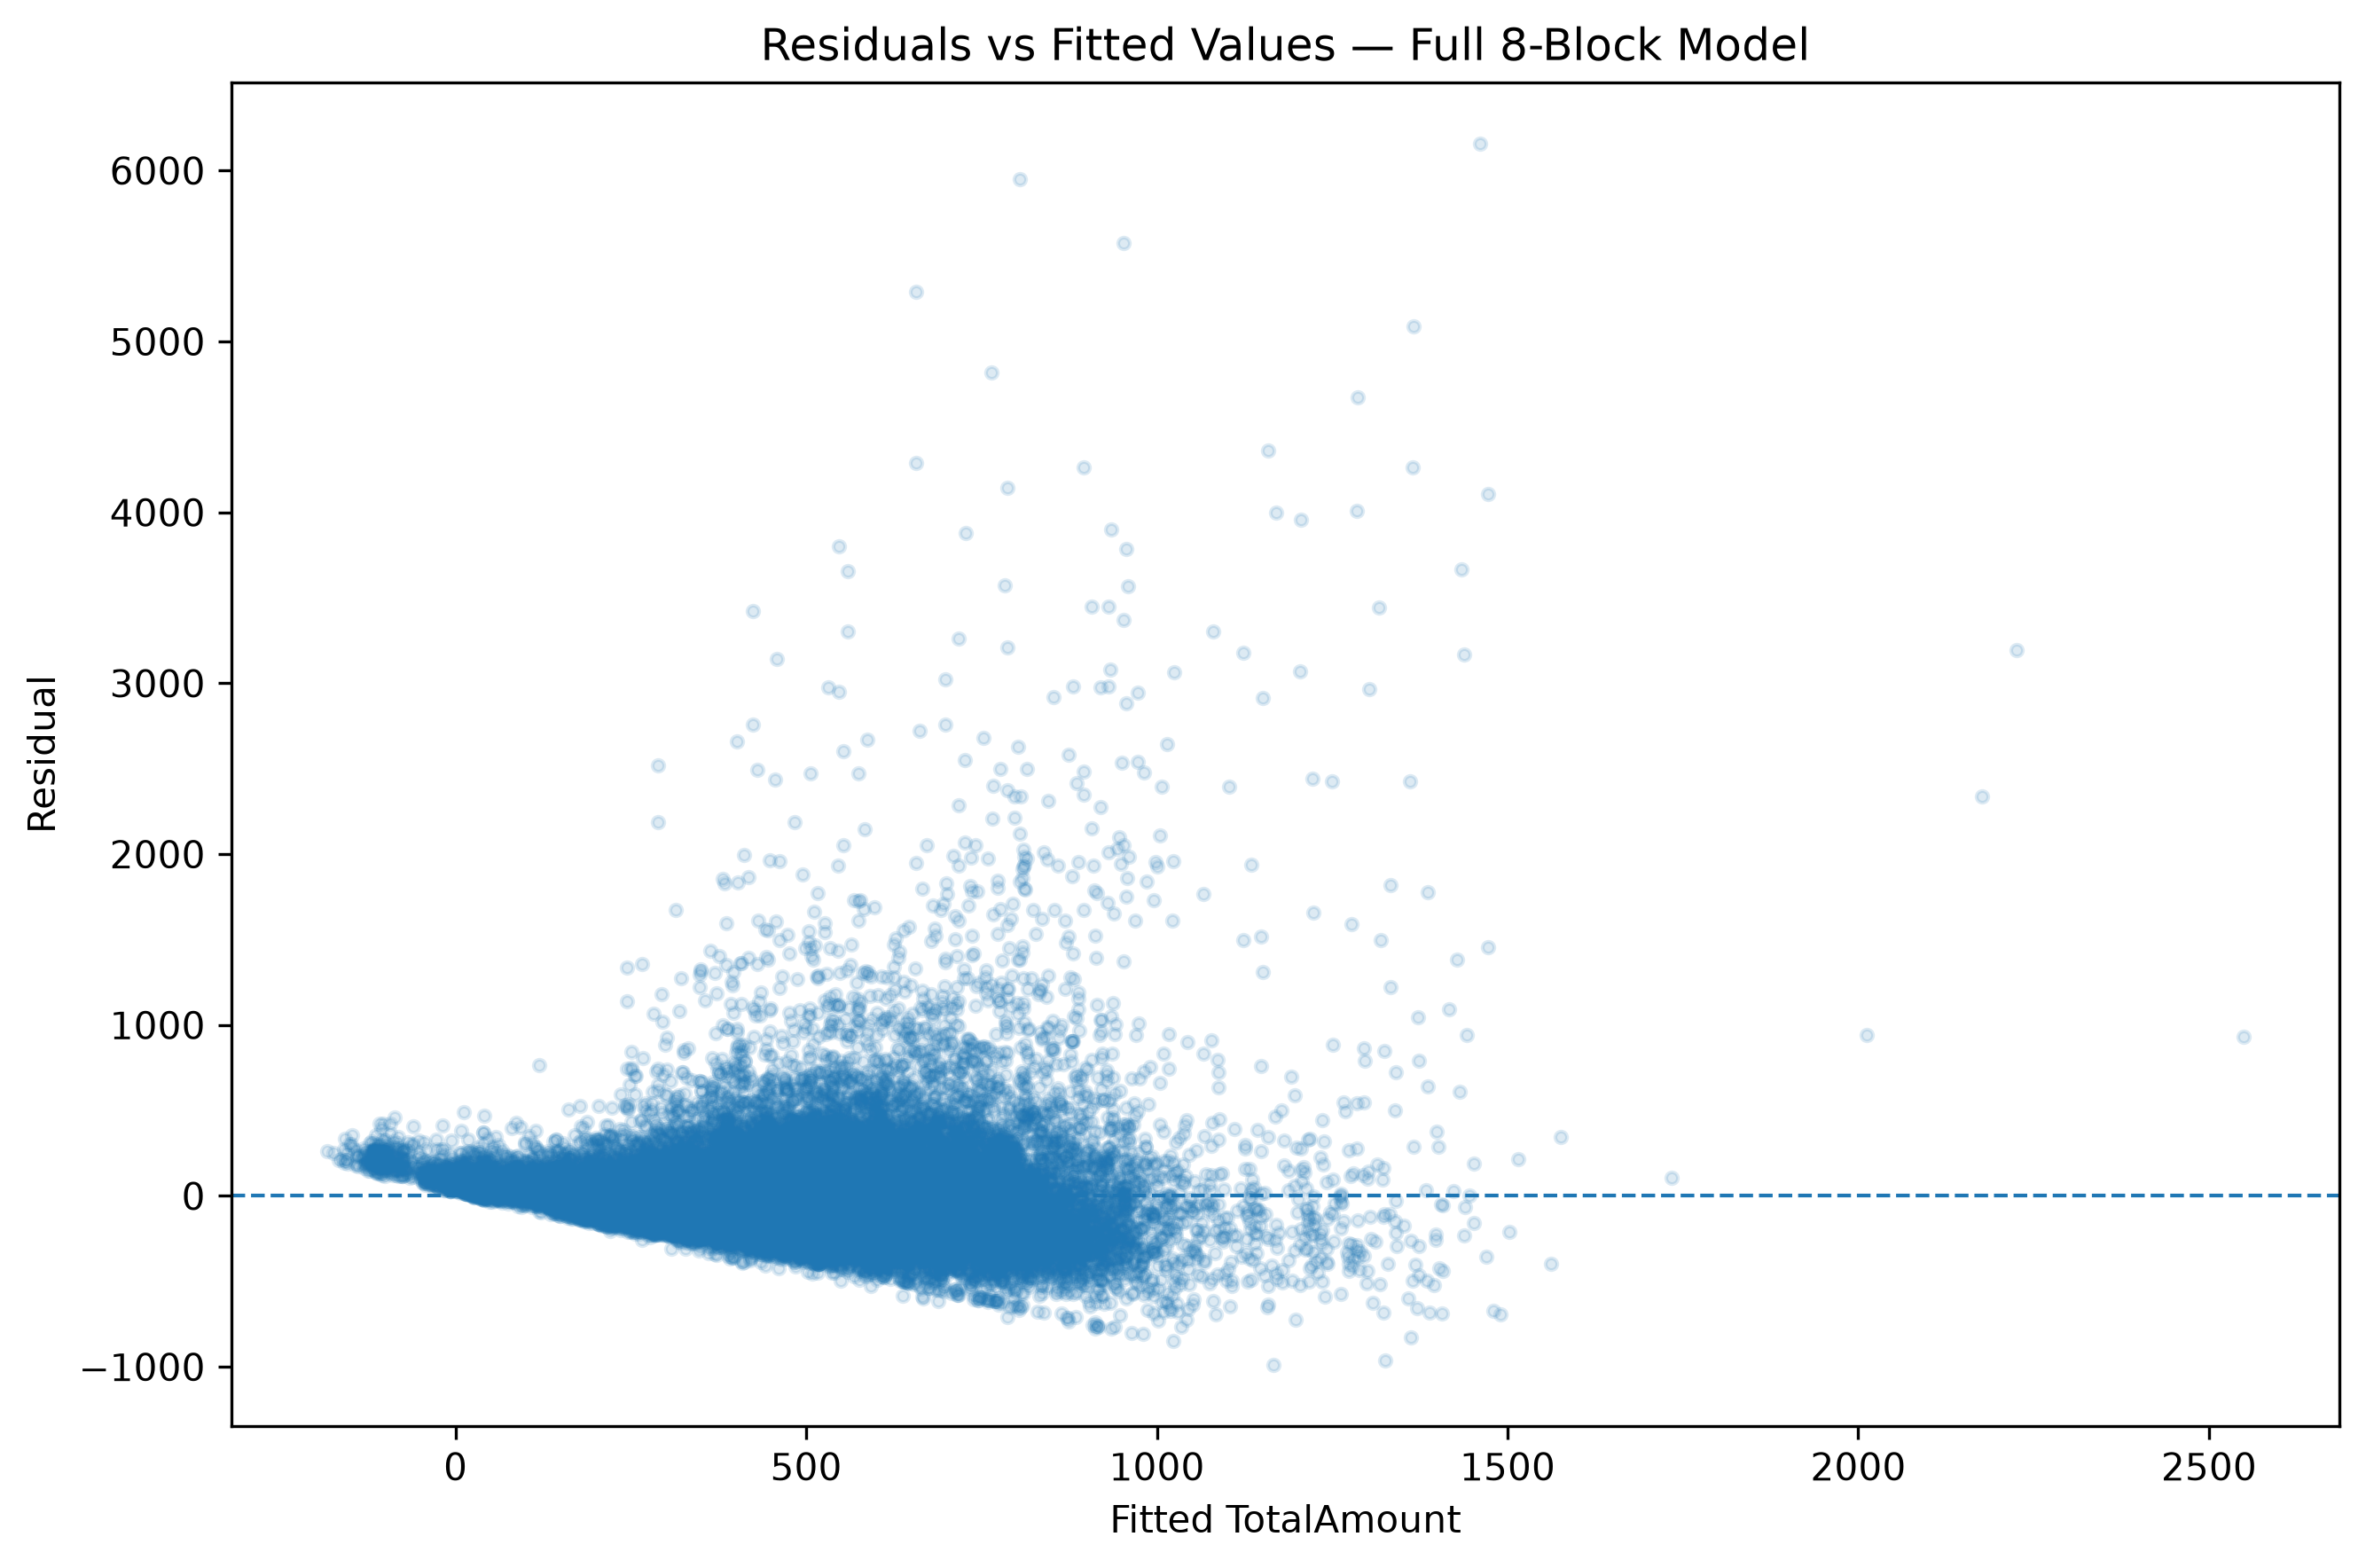
\includegraphics[width=0.78\textwidth]{../outputs/05_full_model_residuals_vs_fitted.png}
\caption{Residuals versus fitted values for the full eight-block level-fare model}
\label{fig:level-residuals-fitted}
\end{figure}

The most prominent feature is a pronounced fan-shaped pattern: residual dispersion increases as the fitted fare rises. This provides clear visual evidence that the constant-error-variance assumption is violated.

The residuals are also asymmetric, with several large positive errors. In addition, a small number of fitted ticket amounts are negative even though the observed response is strictly positive. These features indicate that the level-fare specification requires further refinement.

Partial regression plots for \texttt{TotalDistance} and \texttt{Coupons} do not reveal pronounced curvature. \texttt{TotalDistance} retains a clear positive conditional relationship with fare, while the partial relationship for \texttt{Coupons} is comparatively weak. The main diagnostic concern therefore appears to be the error structure rather than obvious nonlinear functional form in these numerical predictors.

\subsection{Heteroskedasticity and the BLUE Property}

The visual evidence of unequal variance is assessed formally using the Breusch--Pagan test.

\begin{table}[H]
\centering
\caption{Breusch--Pagan tests for the candidate level-fare models}
\label{tab:bp-level-models}
\begin{tabular}{lrr}
\toprule
\textbf{Model} & \textbf{LM statistic} & \textbf{p-value} \\
\midrule
Full eight-block model & 1,590.79 & $<0.001$ \\
Seven-block model & 1,571.32 & $<0.001$ \\
\bottomrule
\end{tabular}
\end{table}

The null hypothesis of constant error variance is strongly rejected for both specifications. The slightly smaller Breusch--Pagan statistic for the seven-block model does not represent a meaningful resolution of the problem; both models continue to exhibit substantial heteroskedasticity.

Under the Gauss--Markov framework, heteroskedasticity has an important implication. If the zero-conditional-mean assumption and the other model assumptions continue to hold, OLS coefficient estimates may remain unbiased and consistent. However, they no longer have minimum variance among linear unbiased estimators.

Therefore, under the current level-fare specification,

\[
\boxed{\text{OLS is not BLUE}}
\]

because the constant-error-variance condition is violated.

This does not imply that the fitted relationships are automatically useless. Rather, it means that the current OLS specification is statistically inefficient and that conventional homoskedastic OLS inference is not appropriate. Remedial modelling is therefore required before the final model is interpreted and validated.

\subsection{Residual Distribution}

The level-fare residuals are also strongly non-normal. Figure~\ref{fig:level-residual-histogram} shows the residual distribution for the full eight-block model.

\begin{figure}[H]
\centering
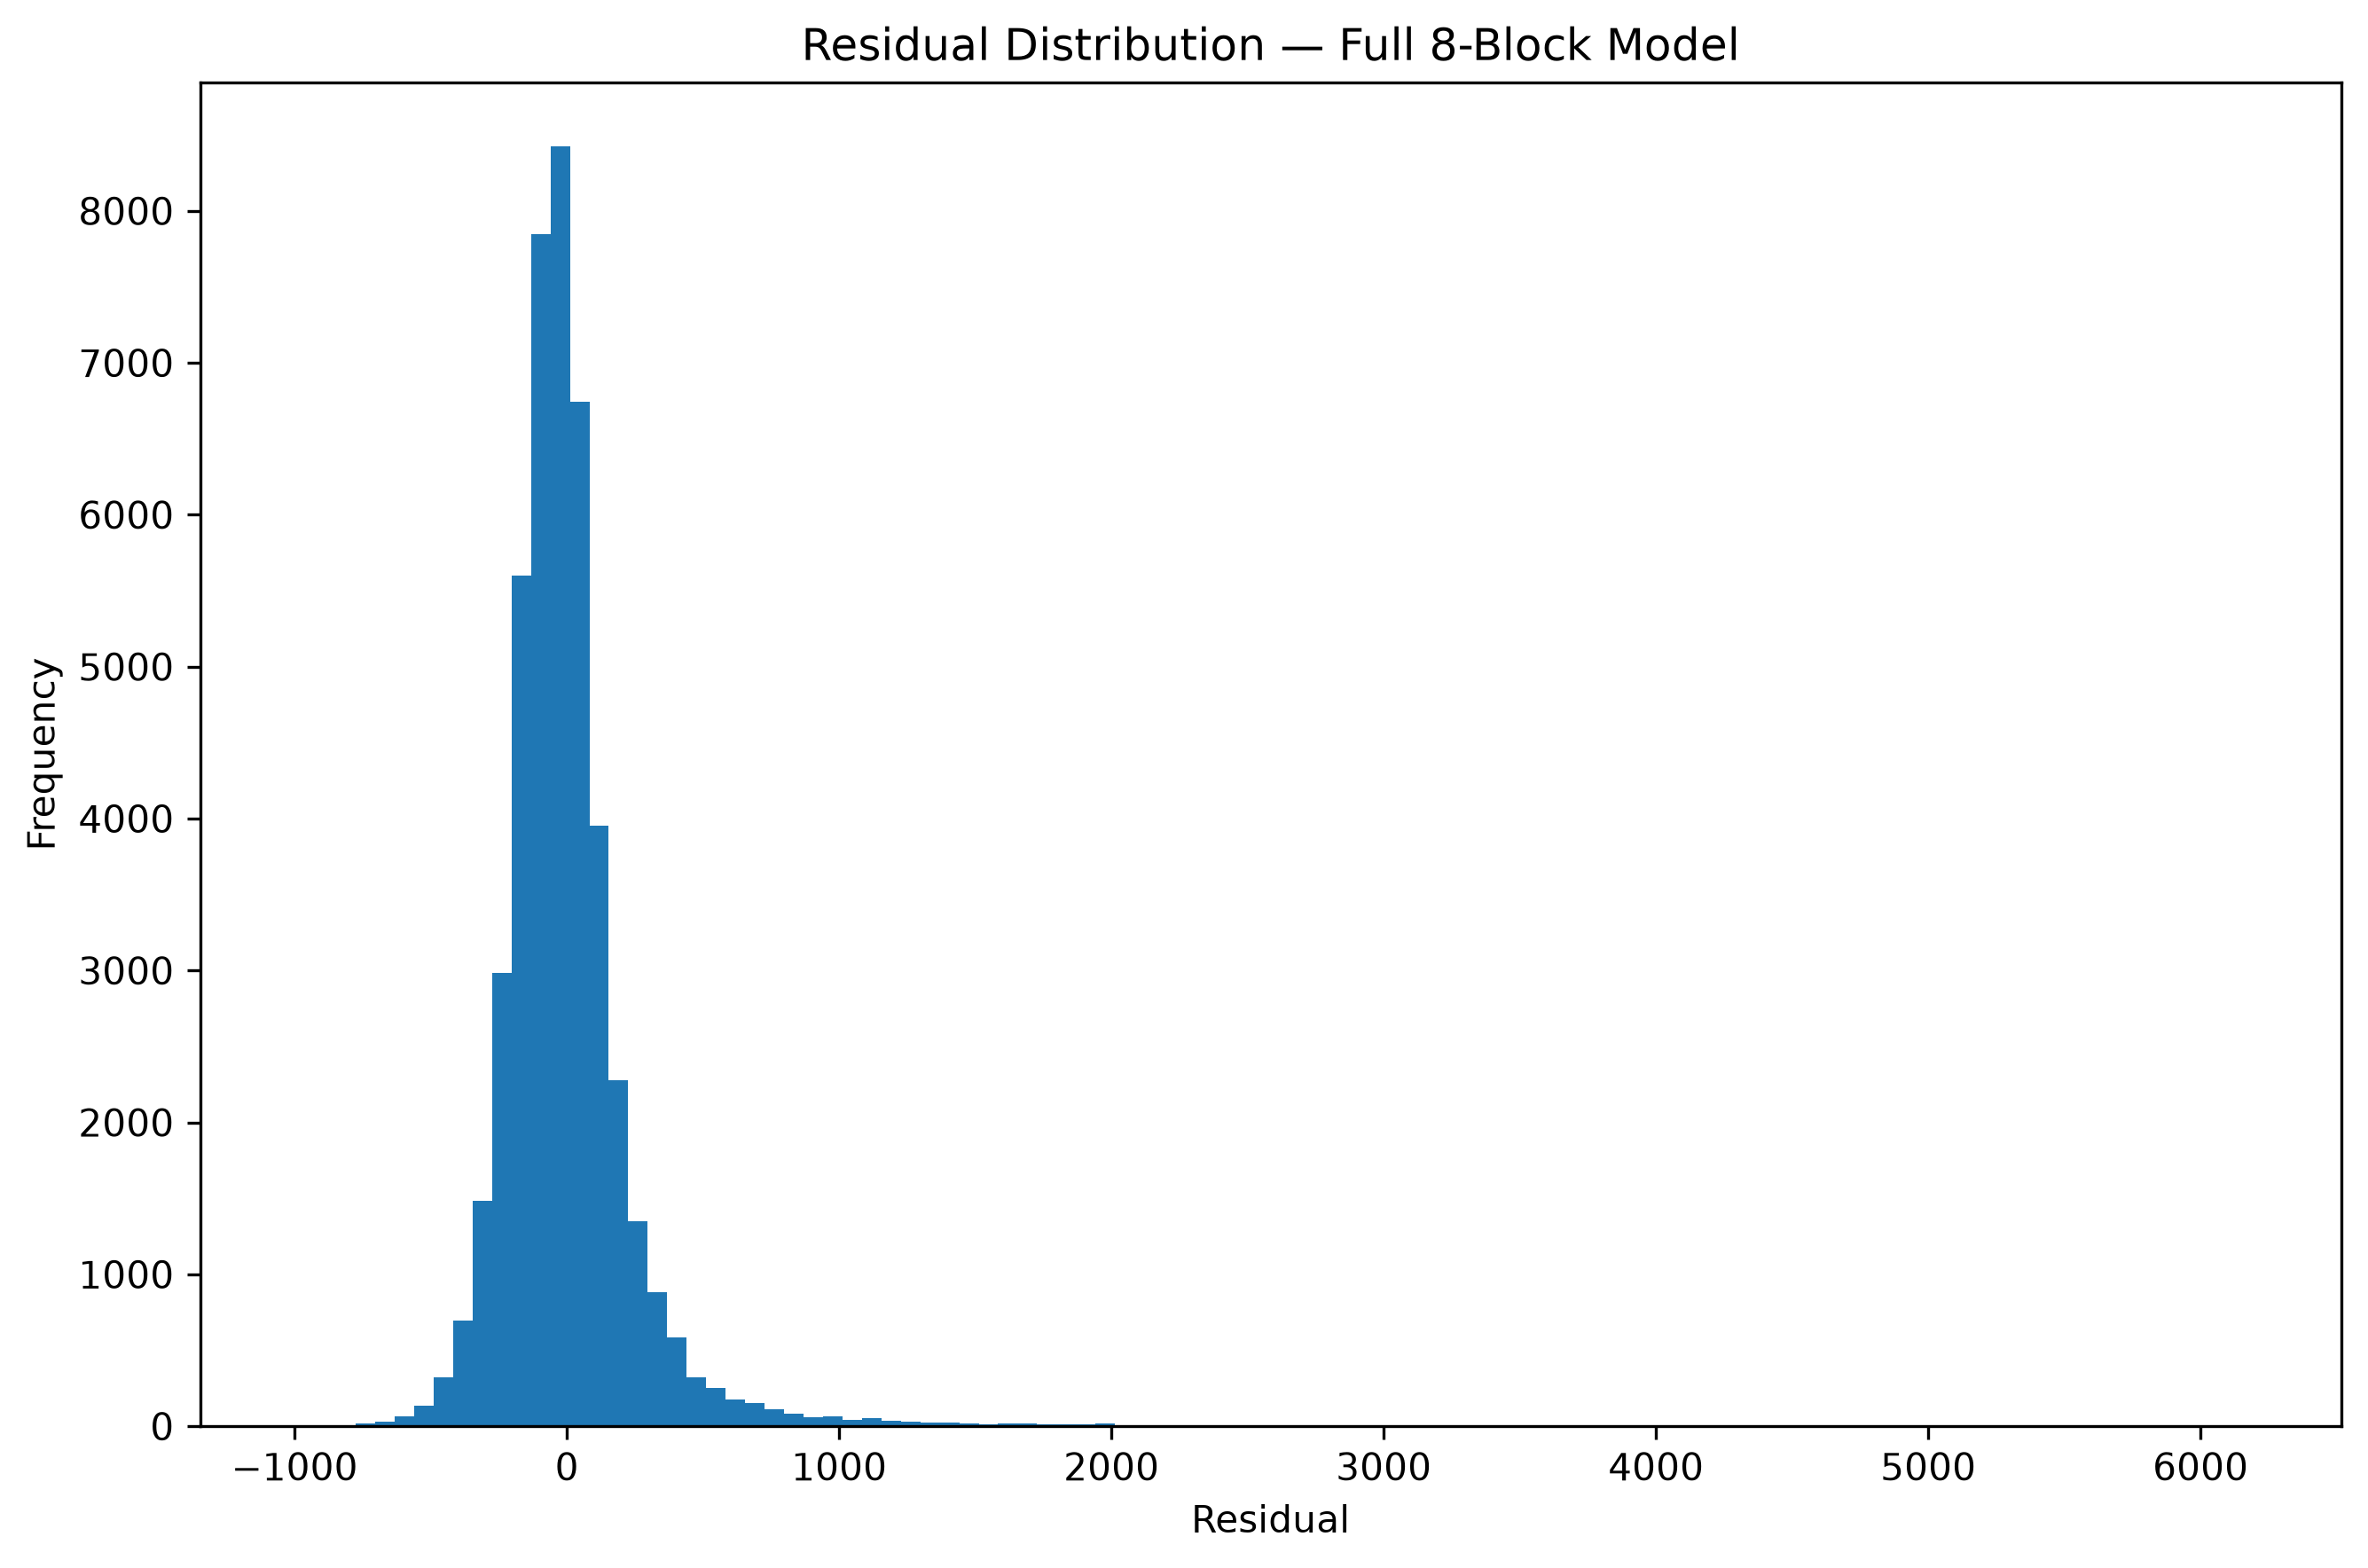
\includegraphics[width=0.78\textwidth]{../outputs/05_full_model_residual_histogram.png}
\caption{Residual distribution for the full eight-block level-fare model}
\label{fig:level-residual-histogram}
\end{figure}

The distribution is strongly right-skewed, with a long positive tail. Normal P--P plots similarly show systematic departures from the normal reference line. The seven-block specification exhibits virtually the same behaviour.

Residual normality is not required for OLS to satisfy the BLUE property, and the large model-building sample reduces the importance of moderate non-normality for asymptotic inference. Nevertheless, the severity of the skewness reinforces the need to reconsider the response specification, particularly because it occurs together with pronounced heteroskedasticity.

\subsection{Outliers, Leverage, and Influence}

Unusual observations are examined using studentized deleted residuals, leverage, DFFITS, Cook's distance, and DFBETAS. These diagnostics do not constitute Gauss--Markov assumptions themselves, but they help determine whether the observed diagnostic problems are driven by a small number of individual cases.

A Bonferroni procedure identifies 254 response outliers in each candidate model, representing approximately 0.56\% of the model-building sample. The Bonferroni critical value is approximately

\[
|t_i| > 4.872,
\]

while the largest absolute studentized deleted residual is approximately 22.44. The most extreme observations are associated primarily with unusually large positive residuals.

Leverage is assessed using the guideline

\[
h_{ii} > \frac{2p}{n}.
\]

This flags 4,602 observations in the full model and 4,676 in the seven-block model. However, the maximum leverage is only approximately 0.014 for both specifications, well below the lecture guidelines of 0.2 for moderate leverage and 0.5 for very high leverage. The relatively large number of flags therefore reflects the very low large-sample threshold rather than widespread extreme leverage.

Table~\ref{tab:influence-summary} summarises the principal influence diagnostics.

\begin{table}[H]
\centering
\caption{Outlier and influence diagnostics for the candidate models}
\label{tab:influence-summary}
\begin{tabular}{lrr}
\toprule
\textbf{Diagnostic} & \textbf{8-block} & \textbf{7-block} \\
\midrule
Bonferroni response outliers & 254 & 254 \\
Maximum $|t_i|$ & 22.44 & 22.44 \\
High-leverage observations & 4,602 & 4,676 \\
Maximum leverage & 0.0141 & 0.0141 \\
DFFITS flags & 1,384 & 1,371 \\
Maximum $|\mathrm{DFFITS}|$ & 1.116 & 1.115 \\
Maximum Cook's distance & 0.0203 & 0.0206 \\
\bottomrule
\end{tabular}
\end{table}

DFFITS identifies a number of locally influential observations, including all 254 Bonferroni response outliers. However, the maximum Cook's distance is only approximately 0.02 for both models. This indicates that no single observation exerts dominant influence over the fitted regression as a whole.

The standard large-sample DFBETAS threshold is extremely small in this dataset, approximately 0.0094, and consequently flags many observations for at least one coefficient. More substantial effects are uncommon: approximately 1.05\% of observations exceed an absolute DFBETAS value of 0.10, 0.22\% exceed 0.20, and only seven observations exceed 0.50. The largest effects are concentrated mainly in carrier and origin-state indicators, together with some sensitivity in \texttt{TotalDistance}.

Overall, the evidence indicates localised influence rather than widespread coefficient instability. Flagged observations are therefore retained rather than deleted mechanically.

\subsection{Independence of Errors}

The observations are cross-sectional ticket records and have no meaningful sequential time ordering. Time-series autocorrelation diagnostics such as the Durbin--Watson and Breusch--Godfrey tests are therefore not appropriate for this dataset.

Error independence cannot be verified directly from the available cross-sectional information and remains a modelling assumption.

\subsection{Diagnostic Comparison of the Candidate Models}

The full eight-block and seven-block specifications are diagnostically almost indistinguishable.

Both models exhibit:

\begin{itemize}
    \item pronounced heteroskedasticity;
    \item strongly right-skewed residuals;
    \item the same 254 Bonferroni response outliers;
    \item similar leverage patterns;
    \item similar DFFITS and Cook's-distance behaviour; and
    \item virtually identical in-sample fit.
\end{itemize}

Removing \texttt{Coupons} therefore does not resolve any of the principal diagnostic problems. The weaknesses appear to arise from the common level-fare specification and error structure rather than from inclusion of this predictor.

\subsection{Implications for Model Refinement}

The diagnostic analysis identifies heteroskedasticity as the most important violation of the level-linear OLS specification, accompanied by pronounced residual skewness. In contrast, severe multicollinearity, obvious curvature in the numerical predictors, and domination by individual influential observations are not evident.

The next modelling stage therefore focuses on the response specification rather than further deleting predictors. In particular, a logarithmic transformation of \texttt{TotalAmount} is investigated to determine whether it improves residual behaviour and variance stability.

The transformed model is then re-diagnosed before further remedies for heteroskedasticity, including weighted least squares and heteroskedasticity-robust inference, are considered.


% ============================================================
% SECTION 7 - MODEL REFINEMENT AND REMEDIAL MEASURES
% ============================================================

\section{Model Refinement and Remedial Measures}

\noindent\textit{Code reference: Notebook 06 (\texttt{06\_model\_refinement.ipynb}).}

The diagnostic analysis in Section 6 identified substantial residual skewness and heteroskedasticity in the level-fare OLS specification. Because removing \texttt{Coupons} did not materially improve these problems, refinement focuses on the response and error structure rather than further variable deletion.

All refinement decisions continue to use only the 45,043-observation model-building sample. The validation sample remains untouched.

\subsection{Logarithmic Transformation of Ticket Fare}

Because ticket fares are strictly positive and strongly right-skewed, the response variable is transformed as

\[
\text{LogTotalAmount}_i = \ln(\text{TotalAmount}_i).
\]

The original eight-block specification is then re-estimated using \texttt{LogTotalAmount} as the response.

The resulting log-response OLS model has

\[
R^2 = 0.5742.
\]

This value refers to variation in log ticket fares and should not be compared directly with the \(R^2\) of the earlier level-fare model because the dependent variable has changed.

Figure~\ref{fig:log-residuals-fitted} shows the residual-versus-fitted pattern after the transformation.

\begin{figure}[H]
\centering
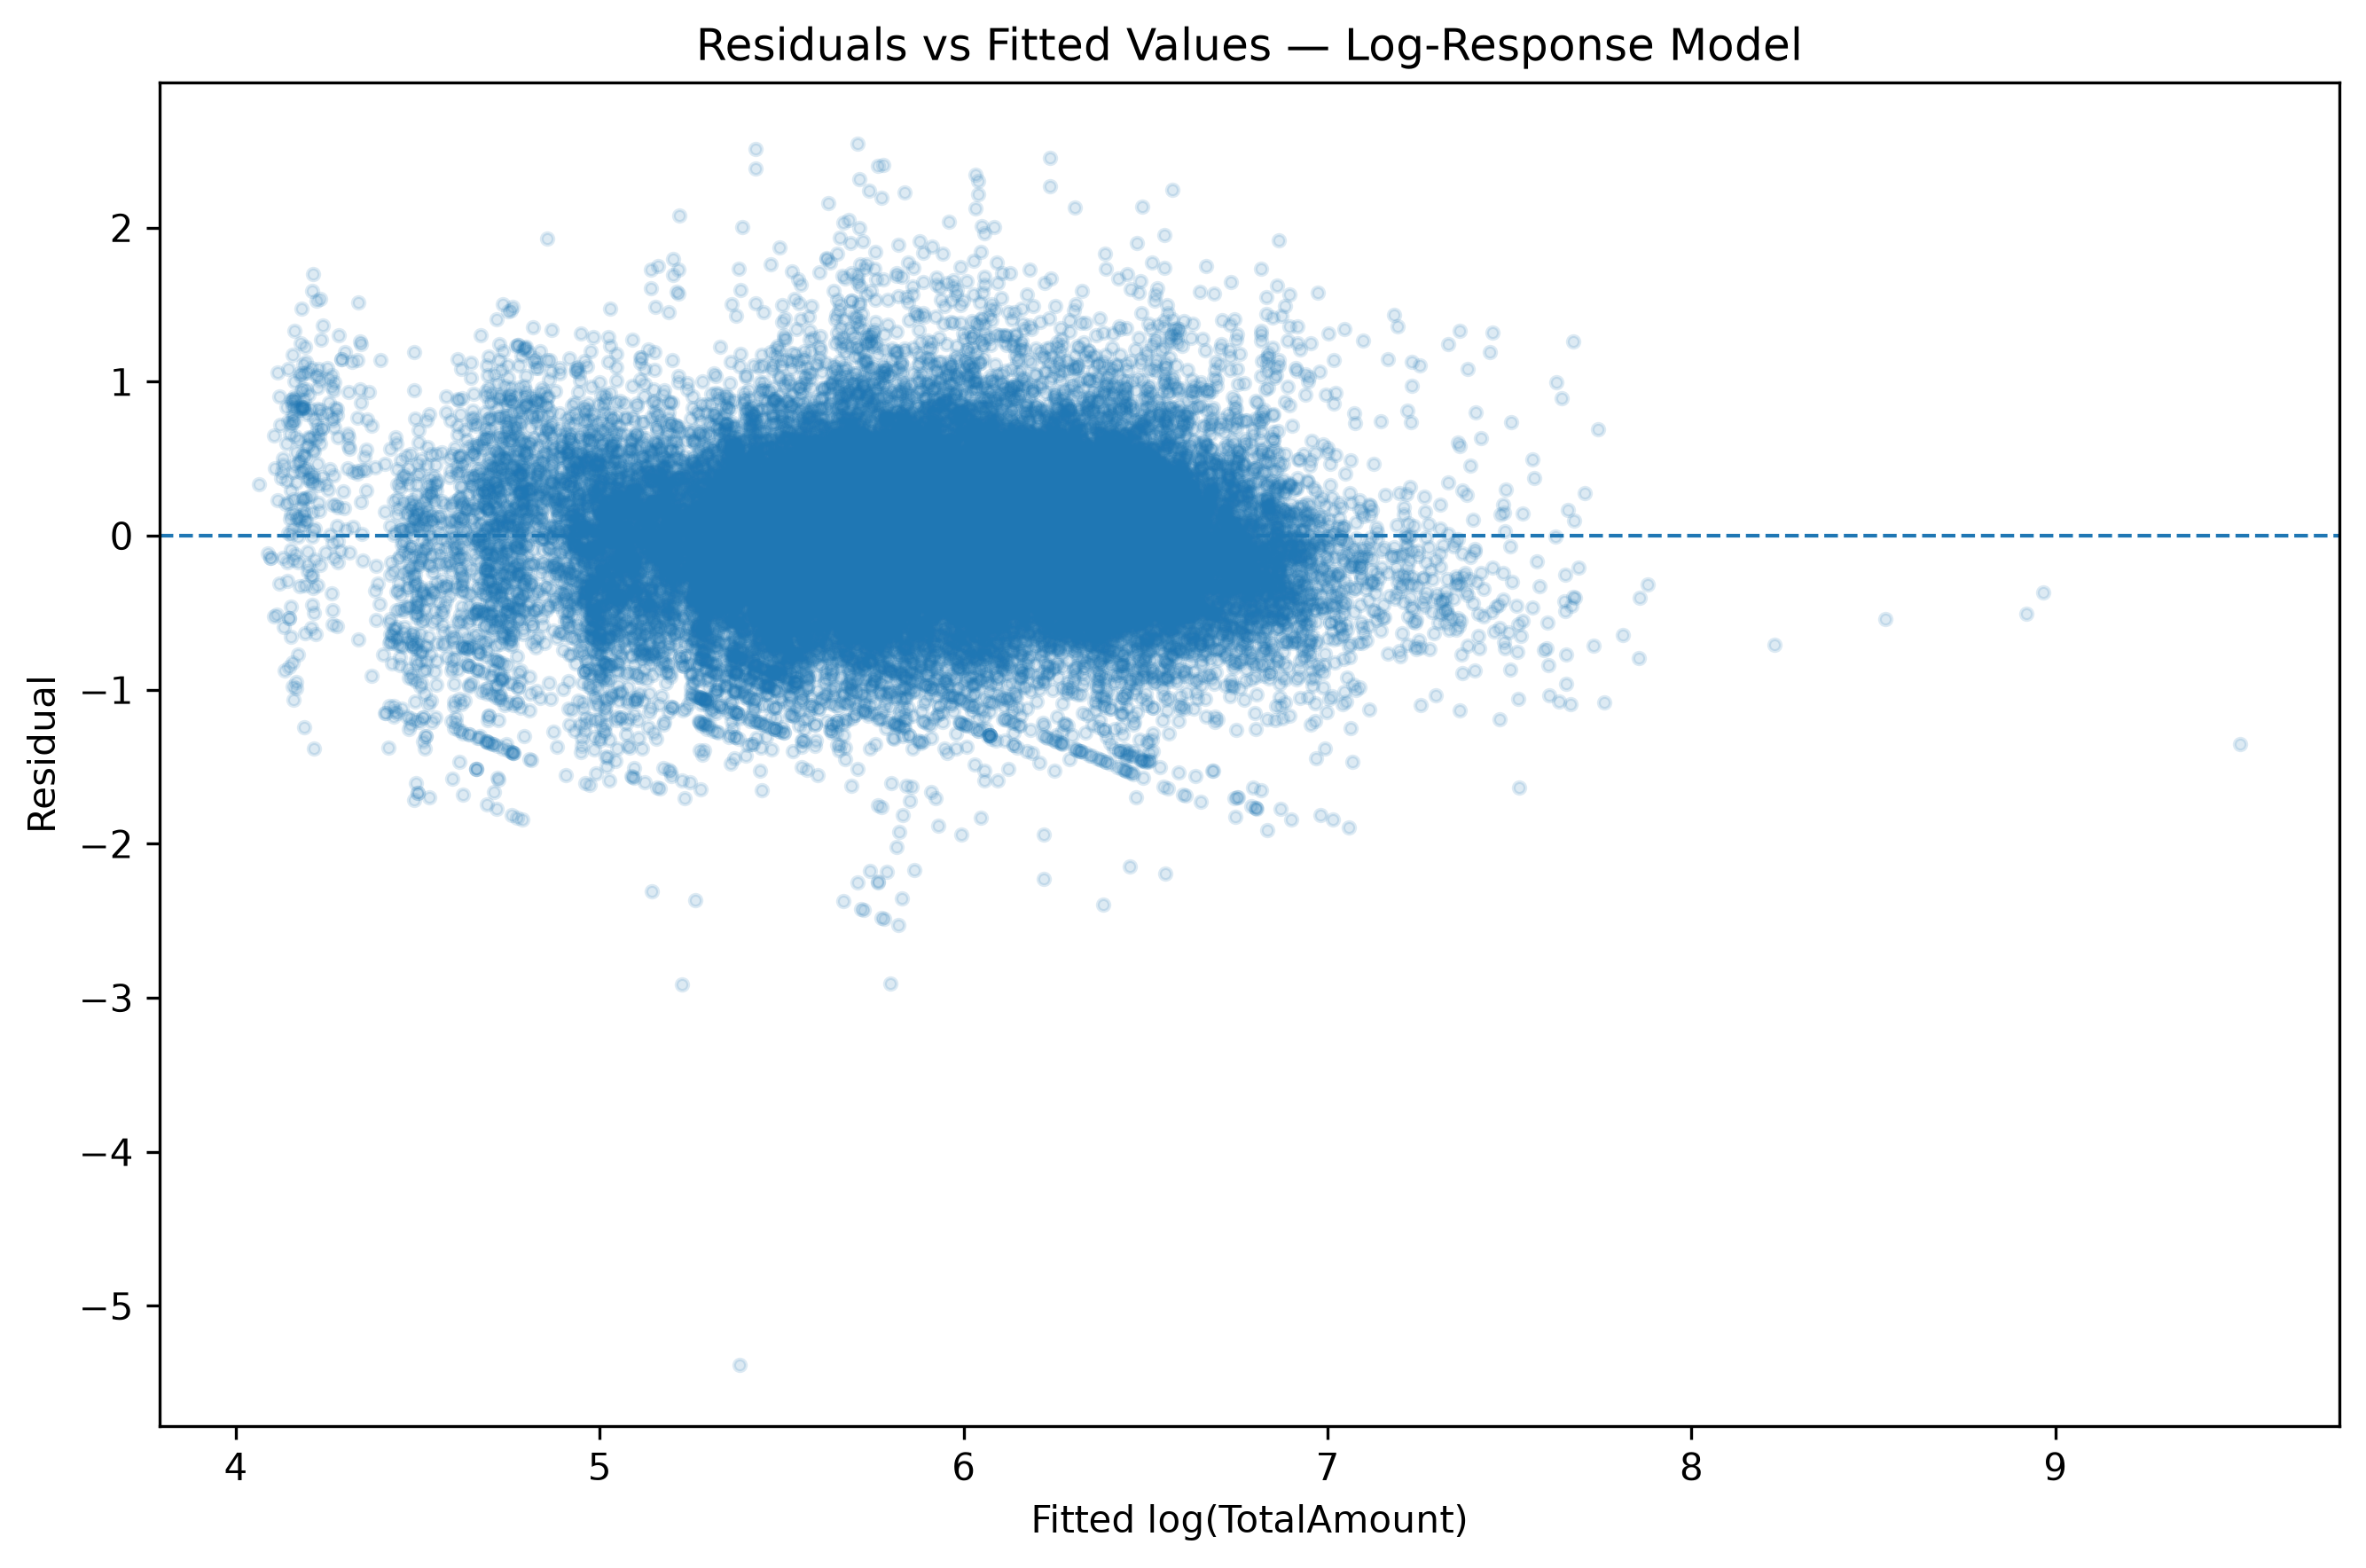
\includegraphics[width=0.78\textwidth]{../outputs/06_log_model_residuals_vs_fitted.png}
\caption{Residuals versus fitted values for the log-response OLS model}
\label{fig:log-residuals-fitted}
\end{figure}

The transformation produces a visibly more balanced residual spread and substantially reduces the pronounced fan shape observed in the level-fare model. The residual distribution also becomes much more symmetric, with the extreme positive tail substantially reduced.

However, the spread is still not constant across fitted values. The Breusch--Pagan test continues to reject homoskedasticity:

\[
LM = 1681.85,
\qquad
p < 0.001.
\]

Thus, the logarithmic transformation substantially improves the residual structure but does not by itself restore constant error variance. Additional treatment of heteroskedasticity is therefore required.

\subsection{Empirical Weighted Least Squares}

Weighted least squares is used to reduce the remaining unequal error variance.

If the conditional standard deviation of the error for observation \(i\) is \(\sigma_i\), efficient WLS assigns weight

\[
w_i = \frac{1}{\sigma_i^2}.
\]

Because the true \(\sigma_i\) is unknown, it must be estimated from the model-building sample. The absolute residuals from the log-response OLS model are used as an empirical proxy for the error standard deviation.

An initial examination of absolute residuals against fitted log fares reveals an approximately U-shaped pattern, with larger residual magnitudes at both the lower and upper ends of the fitted range. This motivates a quadratic approximation:

\[
\widehat{\sigma}_i
=
\gamma_0
+
\gamma_1 \widehat{Y}_i
+
\gamma_2 \widehat{Y}_i^2,
\]

where \(\widehat{Y}_i\) denotes the fitted log fare from the OLS model.

The quadratic standard-deviation function fits the observed pattern better than a purely linear specification, with adjusted \(R^2\) increasing from approximately 0.006 to 0.018. Its fitted standard deviations remain positive, ranging from approximately 0.31 to 1.22, and the implied WLS weights have a maximum-to-minimum ratio of approximately 15.1.

The resulting initial weights are therefore

\[
w_i = \frac{1}{\widehat{\sigma}_i^2}.
\]

\subsection{Initial WLS and Variance-Function Refinement}

The initial WLS model produces coefficient estimates that remain close to those from log OLS. Most coefficient changes are small, indicating that the substantive relationships are not highly sensitive to the weighting scheme.

The weighted residual pattern improves, and the Breusch--Pagan statistic declines from 1681.85 under log OLS to 1233.33 under initial WLS. However, nonconstant variance remains visible and the formal test continues to reject homoskedasticity.

One further refinement of the estimated standard-deviation function is therefore undertaken. In addition to the fitted log fare and its square, the refined function includes variables that help explain remaining residual dispersion:

\[
\begin{aligned}
\widehat{\sigma}_i
={}&
\gamma_0
+\gamma_1 \widehat{Y}_i
+\gamma_2 \widehat{Y}_i^2
+\gamma_3 \text{TotalDistance}_i \\
&+\gamma_4 \text{RoundTrip}_i
+\gamma_5 \text{OnLine}_i.
\end{aligned}
\]

The adjusted \(R^2\) of the auxiliary standard-deviation model increases modestly from approximately 0.018 to 0.023. All fitted standard deviations remain positive, ranging from approximately 0.28 to 1.38, while the resulting weights have a maximum-to-minimum ratio of approximately 23.6.

These estimated weights are then used to fit the refined WLS model.

\subsection{Residual Behaviour Under Refined WLS}

Figure~\ref{fig:refined-wls-residuals} shows the weighted residuals from the refined WLS specification.

\begin{figure}[H]
\centering
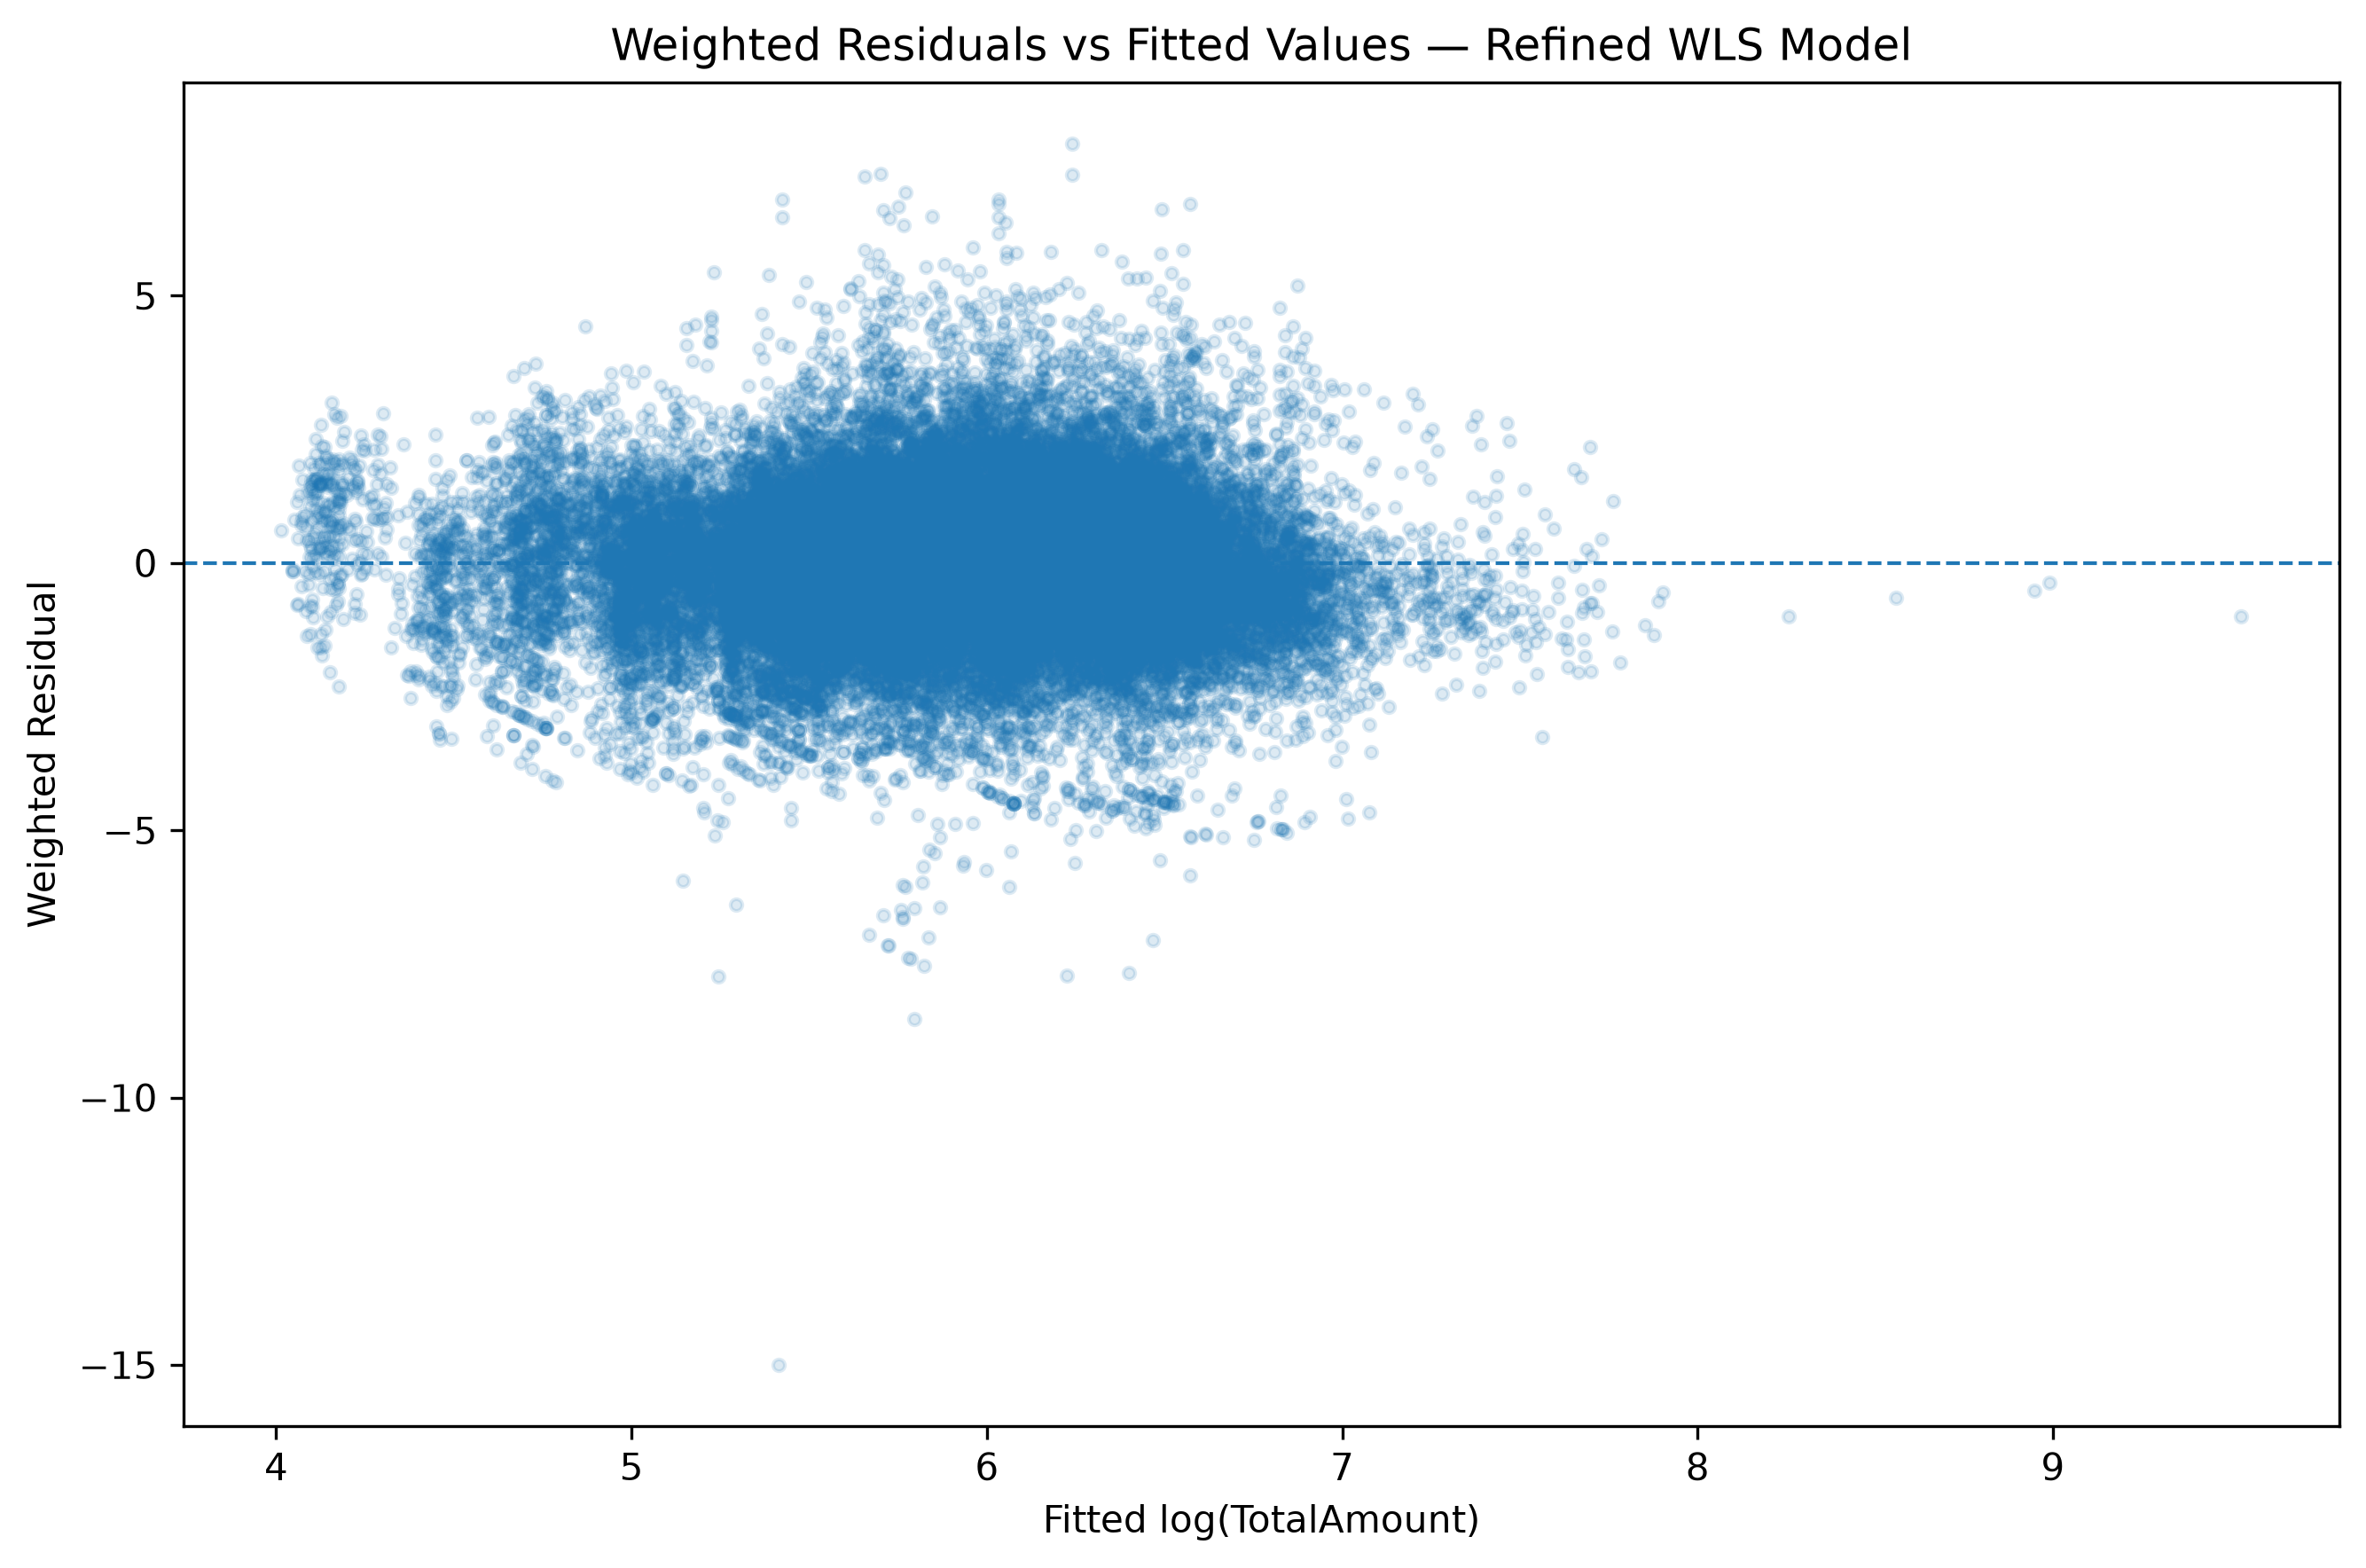
\includegraphics[width=0.78\textwidth]{../outputs/06_refined_wls_weighted_residuals_vs_fitted.png}
\caption{Weighted residuals versus fitted values for the refined WLS model}
\label{fig:refined-wls-residuals}
\end{figure}

The weighted residual spread is more balanced than under either log OLS or the initial WLS specification.

Table~\ref{tab:refinement-bp} summarises the progression in the Breusch--Pagan statistic.

\begin{table}[H]
\centering
\caption{Heteroskedasticity assessment across refinement stages}
\label{tab:refinement-bp}
\begin{tabular}{lrr}
\toprule
\textbf{Model} & \textbf{Breusch--Pagan LM} & \textbf{p-value} \\
\midrule
Log-response OLS & 1681.85 & $<0.001$ \\
Initial WLS & 1233.33 & $<0.001$ \\
Refined WLS & 1003.04 & $<0.001$ \\
\bottomrule
\end{tabular}
\end{table}

The successive reductions in the LM statistic and improvement in the weighted-residual pattern indicate that the WLS procedure materially reduces the unequal variance.

Nevertheless, the Breusch--Pagan test remains statistically significant. With more than 45,000 model-building observations, the test is highly sensitive to remaining departures from constant variance. The objective is therefore not to continue adding complexity until the p-value becomes insignificant, but to obtain a materially improved and interpretable weighting scheme.

No further refinement of the standard-deviation function is pursued.

Because the WLS weights are estimated from the sample rather than based on known error variances, the procedure is an empirical or feasible WLS approach. Exact finite-sample BLUE efficiency therefore cannot be claimed. Refined WLS is instead retained as the primary estimation approach because it substantially improves variance stability relative to the unweighted specification.

\subsection{White-Robust OLS as a Robustness Benchmark}

A second approach to heteroskedasticity is to retain the log-response OLS coefficient estimates but replace the conventional covariance matrix with White heteroskedasticity-robust standard errors.

This method does not remove heteroskedasticity or restore the BLUE property. Instead, it provides inference that is robust to unknown forms of unequal error variance.

The White-corrected log OLS model is therefore used as a robustness benchmark for the refined WLS estimates.

The two approaches produce broadly similar coefficient estimates and inferential conclusions. Of the 61 coefficients, only two have different 5\% significance classifications when refined WLS is compared with OLS using White standard errors, and both are origin-state indicators close to the significance threshold.

Similarly, applying White standard errors rather than conventional OLS standard errors changes the 5\% significance classification of only one coefficient.

The main substantive findings are therefore not driven by the particular WLS weighting scheme.

\subsection{Reassessment of the Candidate Specifications}

Because the response transformation materially changes the fitted model, the earlier variable-selection conclusion is reassessed on the log scale.

Table~\ref{tab:log-candidate-comparison} compares the full eight-block specification with the seven-block alternative that excludes \texttt{Coupons}.

\begin{table}[H]
\centering
\caption{Comparison of the log-response candidate specifications}
\label{tab:log-candidate-comparison}
\begin{tabular}{lrrrrr}
\toprule
\textbf{Specification} & \textbf{Parameters} & \(\mathbf{R^2}\) & \(\mathbf{Adj.\ R^2}\) & \textbf{AIC} & \textbf{BIC} \\
\midrule
Eight-block & 61 & 0.574214 & 0.573646 & 56030.08 & 56561.72 \\
Seven-block, no Coupons & 60 & 0.574123 & 0.573565 & 56037.66 & 56560.58 \\
\bottomrule
\end{tabular}
\end{table}

The two specifications remain extremely similar in overall fit. The eight-block model has slightly higher adjusted \(R^2\) and lower AIC, while BIC marginally favours the seven-block alternative.

Importantly, the behaviour of \texttt{Coupons} changes after transformation and refinement. Under the refined WLS specification,

\[
\hat{\beta}_{\text{Coupons}} = 0.01314,
\qquad
SE = 0.00360,
\qquad
p = 0.00026.
\]

The result is also supported by the White-robust OLS benchmark:

\[
\hat{\beta}_{\text{Coupons}} = 0.01164,
\qquad
SE_{\text{White}} = 0.00373,
\qquad
p = 0.0018.
\]

Thus, \texttt{Coupons} now provides statistically supported explanatory information after the response transformation and remains robust across the two approaches to heteroskedasticity.

The eight-block specification is therefore provisionally preferred. However, because the difference in overall fit is very small and BIC marginally favours the simpler specification, the seven-block model remains a plausible alternative.

Both specifications are carried forward to the held-out validation sample. Final model selection is based on out-of-sample prediction performance, coefficient stability, explanatory value, and parsimony.

% ============================================================
% SECTION 8 - MODEL VALIDATION AND FINAL SELECTION
% ============================================================

\section{Model Validation and Final Selection}

\noindent\textit{Code reference: Notebook 07 (\texttt{07\_model\_validation.ipynb}).}

Following model refinement, two log-response candidate specifications remain:

\begin{enumerate}
    \item the full eight-block model including \texttt{Coupons}; and
    \item the reduced seven-block model excluding \texttt{Coupons}.
\end{enumerate}

Both specifications are estimated using the same refined weighted least squares procedure. The validation exercise therefore isolates the contribution of the additional \texttt{Coupons} predictor rather than differences in estimation method.

The original 50/50 model-building and validation split is reproduced exactly. All categorical grouping rules and variance-function forms are determined exclusively from the model-building sample. No new variable selection, transformation, or variance-function refinement is performed using the validation observations.

\subsection{Out-of-Sample Prediction Performance}

Prediction performance is assessed using mean squared prediction error:

\[
MSPR=\frac{1}{n^*}\sum_{i=1}^{n^*}\left(Y_i-\hat{Y}_i\right)^2,
\]

where \(Y_i\) is the observed log fare in the validation sample and \(\hat{Y}_i\) is the prediction obtained from the model fitted using the model-building sample.

The resulting MSPRs are:

\[
MSPR_{\text{8-block}}=0.206064,
\]

and

\[
MSPR_{\text{7-block}}=0.206112.
\]

The difference is only approximately 0.02\%, indicating that the two candidate specifications have essentially identical out-of-sample predictive performance.

To assess whether predictive performance deteriorates materially outside the model-building sample, validation MSPR is also compared with training MSE.

\begin{table}[H]
\centering
\caption{Training and validation performance of the candidate models}
\label{tab:validation-performance}
\begin{tabular}{lrrrr}
\toprule
\textbf{Specification} & \textbf{Training MSE} & \textbf{Validation MSE} & \textbf{Validation MSPR} & \textbf{MSPR/MSE gap} \\
\midrule
Eight-block & 0.203005 & 0.205866 & 0.206064 & 1.51\% \\
Seven-block & 0.203042 & 0.205907 & 0.206112 & 1.51\% \\
\bottomrule
\end{tabular}
\end{table}

For both specifications, validation MSPR is only approximately 1.5\% higher than training MSE. This small deterioration indicates that both models maintain similar predictive performance on unseen observations and provides no evidence of material overfitting.

The eight-block model performs marginally better on both training MSE and validation MSPR, but the differences are too small to provide a strong basis for model selection on prediction error alone.

\subsection{Training and Validation Explanatory Fit}

Adjusted \(R^2\) is also compared across the two candidate specifications and across samples.

\begin{table}[H]
\centering
\caption{Adjusted \(R^2\) across model-building and validation samples}
\label{tab:validation-adjusted-r2}
\begin{tabular}{lrr}
\toprule
\textbf{Specification} & \textbf{Model-building} & \textbf{Validation} \\
\midrule
Eight-block & 0.573313 & 0.568462 \\
Seven-block & 0.573235 & 0.568375 \\
\bottomrule
\end{tabular}
\end{table}

Both models experience only a small decline in adjusted \(R^2\) between the model-building and validation samples. The eight-block specification falls from approximately 0.573 to 0.568, while the seven-block specification exhibits almost the same change.

This consistency provides further evidence that the fitted relationships generalise reasonably well to independent observations. The eight-block specification retains a marginally higher adjusted \(R^2\) in both samples, although the differences remain very small.

\subsection{Coefficient Stability}

The candidate specifications are also re-estimated on the validation sample using the corresponding variance functions estimated from the model-building sample. These validation refits are used only to assess coefficient stability; out-of-sample MSPR continues to be calculated using predictions from the original model-building models.

Table~\ref{tab:coefficient-stability} summarises the stability of the coefficient estimates.

\begin{table}[H]
\centering
\caption{Coefficient stability across model-building and validation samples}
\label{tab:coefficient-stability}
\begin{tabular}{lrrr}
\toprule
\textbf{Specification} & \textbf{Median absolute change} & \textbf{Maximum absolute change} & \textbf{Sign changes} \\
\midrule
Eight-block & 0.0157 & 0.0666 & 3 \\
Seven-block & 0.0159 & 0.0673 & 3 \\
\bottomrule
\end{tabular}
\end{table}

The two candidate specifications exhibit almost identical coefficient stability.

Each model contains three sign changes, involving the Arizona, New Jersey, and Oregon origin-state coefficients. These apparent reversals are not economically meaningful. In both samples, the coefficients are small and statistically insignificant, indicating that their estimated effects fluctuate around zero rather than representing genuine instability.

For example, in the eight-block model the Arizona coefficient changes from 0.0092 in the model-building sample to \(-0.0191\) in the validation sample, while the corresponding p-values are 0.504 and 0.167. Similar behaviour is observed for New Jersey and Oregon.

The economically important coefficients therefore remain broadly stable in sign and magnitude across the two independent samples.

\subsection{Stability of the Additional Predictor}

Because \texttt{Coupons} is the only predictor distinguishing the two candidate specifications, its stability is examined directly.

\begin{table}[H]
\centering
\caption{Stability of the \texttt{Coupons} coefficient}
\label{tab:coupons-validation}
\begin{tabular}{lrrr}
\toprule
\textbf{Sample} & \textbf{Estimate} & \textbf{Standard error} & \textbf{p-value} \\
\midrule
Model-building & 0.013140 & 0.003598 & 0.000260 \\
Validation & 0.012994 & 0.003637 & 0.000354 \\
\bottomrule
\end{tabular}
\end{table}

The \texttt{Coupons} coefficient is highly stable across samples. Its estimate changes only from 0.01314 to 0.01299, while the standard error remains approximately 0.0036.

It is also statistically significant in both samples at well below the 1\% level.

This evidence differs from the initial level-fare OLS specification, where \texttt{Coupons} was not statistically significant. After the response transformation and WLS refinement, the relationship becomes statistically supported and remains highly stable when evaluated using independent observations.

\subsection{Final Model Selection}

The validation results leave both candidate specifications statistically defensible.

The seven-block model has the advantage of slightly greater parsimony, and its out-of-sample performance is virtually indistinguishable from that of the eight-block model. If prediction alone were the objective, the simpler model would therefore be difficult to reject.

However, the purpose of this study is also explanatory. \texttt{Coupons} captures a distinct economic feature of the itinerary---the number of ticketed segments and therefore itinerary complexity. Its coefficient is stable across the model-building and validation samples, statistically significant in both samples, and adds only one estimated parameter.

The eight-block model also produces marginally lower training MSE, validation MSE, and MSPR, together with marginally higher adjusted \(R^2\) in both samples. Although these differences are too small to justify selection on their own, there is no evidence that retaining \texttt{Coupons} harms out-of-sample performance.

The full eight-block specification is therefore selected as the final model.

The retained predictor blocks are:

\begin{itemize}
    \item \texttt{TotalDistance};
    \item \texttt{Coupons};
    \item \texttt{RoundTrip};
    \item \texttt{OnLine};
    \item \texttt{PurchaseWindowGroup};
    \item \texttt{RpCarrier\_Model};
    \item \texttt{ItinGeoType}; and
    \item \texttt{OriginState\_Model}.
\end{itemize}

Refined WLS is retained as the primary estimation approach.

Because the WLS weights are estimated rather than known and some residual heteroskedasticity remains, exact finite-sample BLUE efficiency cannot be claimed. Nevertheless, the final specification demonstrates stable coefficient estimates, little deterioration in out-of-sample performance, and economically interpretable relationships. These results support its use as an exploratory explanatory model and as the basis for the fare-benchmarking application developed in the next section.

% ============================================================
% SECTION 9 - ECONOMIC INTERPRETATION AND FARE BENCHMARKING
% ============================================================

\section{Economic Interpretation and Fare Benchmarking}

\noindent\textit{Code reference: Notebook 08 (\texttt{08\_business\_application.ipynb}).}

Following validation, the selected eight-block log-response specification is re-estimated using the full sample of 90,086 observations. The previously validated carrier and origin-state groupings are retained unchanged, and no further variable selection or model refinement is conducted.

The validated refined-WLS variance-function form is also retained, although its coefficients are re-estimated using the full sample. This allows all available observations to contribute to the final parameter estimates without altering the specification that was selected and validated previously.

The final model contains 61 estimated parameters. All economic interpretations in this section use the resulting full-sample WLS estimates.

\subsection{Interpreting the Log-Response Model}

Because the dependent variable is the logarithm of total ticket amount, coefficients are converted into percentage fare differences.

For a dummy or categorical coefficient \(\beta\), the exact percentage difference relative to the reference category is

\[
100\left(e^\beta-1\right)\%.
\]

For a continuous predictor, the percentage difference associated with a change of \(\Delta x\) units is

\[
100\left(e^{\beta \Delta x}-1\right)\%.
\]

These quantities describe conditional associations after controlling for the remaining variables in the model. They should not be interpreted as causal effects.

\subsection{Itinerary and Purchase Characteristics}

Table~\ref{tab:main-economic-effects} summarises the principal itinerary and purchase effects.

\begin{table}[H]
\centering
\caption{Estimated fare differences for principal itinerary and purchase characteristics}
\label{tab:main-economic-effects}
\begin{tabular}{lr}
\toprule
\textbf{Comparison} & \textbf{Estimated fare difference} \\
\midrule
Additional 100 miles of itinerary distance & +1.58\% \\
Additional 500 miles of itinerary distance & +8.14\% \\
Additional ticket coupon & +1.32\% \\
Round trip vs.\ one way & +55.20\% \\
\texttt{OnLine = 0} vs.\ \texttt{OnLine = 1} & +10.40\% \\
Purchase window \texttt{2290} vs.\ \texttt{21AP} & -26.52\% \\
Purchase window \texttt{91UP} vs.\ \texttt{21AP} & -27.19\% \\
Non-contiguous vs.\ contiguous domestic itinerary & +7.19\% \\
\bottomrule
\end{tabular}
\end{table}

Travel distance is positively associated with fare after controlling for the remaining characteristics. An additional 100 itinerary miles is associated with approximately a 1.58\% higher fare, while a 500-mile increase corresponds to approximately 8.14\%.

Itinerary complexity also contributes additional information. Each additional ticket coupon, representing an additional ticketed segment, is associated with approximately a 1.32\% higher fare. Although this effect is modest, its stability across the model-building and validation samples provides the explanatory justification for retaining \texttt{Coupons} in the final specification.

Round-trip itineraries are associated with approximately 55.20\% higher total ticket amounts than otherwise comparable one-way itineraries. This relatively large difference should be interpreted in the context of the response variable representing the total amount paid for the complete ticket itinerary rather than as a causal round-trip price premium.

Itineraries with \texttt{OnLine = 0} are associated with approximately 10.40\% higher fares than the \texttt{OnLine = 1} reference group.

Purchase timing is also economically important. Relative to the \texttt{21AP} reference category, the \texttt{2290} and \texttt{91UP} categories are associated with fares approximately 26.52\% and 27.19\% lower, respectively.

Finally, non-contiguous domestic itineraries are associated with fares approximately 7.19\% higher than contiguous domestic itineraries after controlling for the remaining observed characteristics.

\subsection{Carrier Effects}

Carrier identity remains strongly associated with fare after controlling for itinerary structure, purchase timing, and geography. American Airlines (\texttt{AA}) is the reference carrier.

\begin{table}[H]
\centering
\caption{Conditional carrier fare differences relative to American Airlines}
\label{tab:carrier-effects}
\begin{tabular}{lrr}
\toprule
\textbf{Carrier} & \textbf{Coefficient} & \textbf{Fare difference vs.\ AA} \\
\midrule
DL & 0.0543 & +5.58\% \\
UA & 0.0236 & +2.39\% \\
WN & -0.0844 & -8.09\% \\
AS & -0.1217 & -11.46\% \\
B6 & -0.2752 & -24.06\% \\
Other & -0.4076 & -33.47\% \\
SY & -0.5979 & -45.01\% \\
MX & -0.7127 & -50.97\% \\
F9 & -0.7469 & -52.62\% \\
XP & -0.9874 & -62.75\% \\
G4 & -1.2924 & -72.54\% \\
\bottomrule
\end{tabular}
\end{table}

Relative to \texttt{AA}, Delta (\texttt{DL}) and United (\texttt{UA}) are associated with fares approximately 5.58\% and 2.39\% higher, respectively. Southwest (\texttt{WN}) and Alaska (\texttt{AS}) are associated with fares approximately 8.09\% and 11.46\% lower.

Larger negative differences are observed for several other carriers. For example, \texttt{B6} is associated with fares approximately 24.06\% lower than \texttt{AA}, while \texttt{F9}, \texttt{XP}, and \texttt{G4} exhibit substantially lower conditional fare levels.

All carrier coefficients shown above are statistically significant at conventional levels. However, these estimates should not be interpreted as causal carrier effects. They may also capture unobserved differences in route mix, service characteristics, fare class, competition, or other factors not fully represented in the model. The \texttt{Other} category represents a pooled group of low-frequency carriers rather than a single airline.

\subsection{Geographic Effects}

Geography remains relevant even after controlling for distance, itinerary structure, purchase characteristics, and carrier identity.

As noted above, non-contiguous domestic itineraries are associated with fares approximately 7.19\% higher than contiguous domestic itineraries.

Origin-state effects are measured relative to California. Table~\ref{tab:selected-state-effects} reports selected estimates illustrating the range of conditional geographic differences.

\begin{table}[H]
\centering
\caption{Selected origin-state fare differences relative to California}
\label{tab:selected-state-effects}
\begin{tabular}{lrrr}
\toprule
\textbf{Origin state} & \textbf{Coefficient} & \textbf{Fare difference} & \textbf{p-value} \\
\midrule
Alabama & 0.1615 & +17.52\% & $<0.001$ \\
Alaska & 0.1441 & +15.50\% & $<0.001$ \\
Minnesota & 0.1423 & +15.30\% & $<0.001$ \\
Oklahoma & 0.1313 & +14.04\% & $<0.001$ \\
Arkansas & 0.1309 & +13.98\% & $<0.001$ \\
\addlinespace
New York & -0.0464 & -4.53\% & $<0.001$ \\
Illinois & -0.0565 & -5.49\% & $<0.001$ \\
Puerto Rico & -0.0979 & -9.33\% & $<0.001$ \\
Hawaii & -0.2993 & -25.87\% & $<0.001$ \\
\bottomrule
\end{tabular}
\end{table}

Several origin states therefore exhibit economically meaningful fare differences relative to California even after the other observable ticket characteristics are held fixed.

Not every state coefficient is statistically distinguishable from California. For example, the estimates for New Jersey, Oregon, Washington, Arizona, Nevada, Idaho, and Maine are not significant at the 5\% level.

The state effects should therefore be interpreted as conditional geographic associations rather than intrinsic state-level price effects. They may partly reflect unobserved differences in route networks, airport structure, competition, or market composition.

\subsection{Fare-Benchmarking Framework}

The final model can also be translated into a practical fare benchmark.

For ticket \(i\), the fitted model first generates a predicted log fare:

\[
\widehat{\log(\text{Fare}_i)}
=
X_i\hat{\beta}.
\]

Exponentiating this value gives the model-implied benchmark on the original dollar scale:

\[
\widehat{\text{Fare}}_i
=
\exp\left(X_i\hat{\beta}\right).
\]

Because the regression is estimated on the logarithmic scale, this retransformed quantity should be interpreted as a typical conditional fare rather than an exact estimate of the arithmetic conditional mean.

For each ticket, the dollar fare gap is defined as

\[
\text{Fare Gap}_i
=
\text{Observed Fare}_i
-
\text{Benchmark Fare}_i,
\]

and the percentage fare gap is

\[
\text{Fare Gap \%}_i
=
\left(
\frac{\text{Observed Fare}_i}
{\text{Benchmark Fare}_i}
-1
\right)
\times 100.
\]

A positive fare gap indicates that the observed ticket is priced above the model-implied benchmark for its observable characteristics, while a negative gap indicates that it is priced below the benchmark.

\subsection{Benchmark Performance on the Full Sample}

Table~\ref{tab:benchmark-summary} compares the observed and model-implied fare distributions.

\begin{table}[H]
\centering
\caption{Summary of observed and model-implied fares}
\label{tab:benchmark-summary}
\begin{tabular}{lrrr}
\toprule
\textbf{Statistic} & \textbf{Observed fare} & \textbf{Benchmark fare} & \textbf{Fare gap (\%)} \\
\midrule
Mean & \$460.01 & \$421.31 & 10.64\% \\
25th percentile & \$242.20 & \$267.05 & -23.44\% \\
Median & \$388.40 & \$378.17 & -0.26\% \\
75th percentile & \$580.30 & \$540.25 & 29.94\% \\
\bottomrule
\end{tabular}
\end{table}

The benchmark is well centred for a typical observation. The median observed fare is \$388.40 compared with a median model-implied benchmark of \$378.17, while the median percentage gap is only -0.26\%.

The mean observed fare exceeds the mean benchmark because the observed fare distribution remains right-skewed and exponentiating the predicted log fare does not estimate the arithmetic conditional mean.

Substantial residual variation nevertheless remains. The middle 50\% of tickets lie approximately between 23.44\% below and 29.94\% above their respective benchmarks. This is consistent with the fact that airline fares are also influenced by characteristics not observed in the dataset.

\subsection{Illustrative Fare Comparisons}

For illustration, tickets within 25\% of their model-implied benchmark are classified as \textit{near benchmark}. Tickets more than 25\% below or above the benchmark are labelled \textit{relatively low} or \textit{relatively high}, respectively.

These thresholds are descriptive and are not statistical significance cutoffs.

Across the full sample:

\begin{itemize}
    \item 43,582 tickets, or approximately 48.38\%, are within 25\% of their benchmark;
    \item 21,069 tickets, or approximately 23.39\%, are more than 25\% below their benchmark; and
    \item 25,435 tickets, or approximately 28.23\%, are more than 25\% above their benchmark.
\end{itemize}

Table~\ref{tab:benchmark-examples} provides three representative examples.

\begin{table}[H]
\centering
\caption{Illustrative fare-benchmarking examples}
\label{tab:benchmark-examples}
\small
\begin{tabular}{lrrrrlll}
\toprule
\textbf{Classification} & \textbf{Observed} & \textbf{Benchmark} & \textbf{Gap} & \textbf{Miles} & \textbf{Carrier} & \textbf{Window} & \textbf{State} \\
\midrule
Relatively low & \$142.99 & \$204.27 & -30.0\% & 1,276 & MX & 2290 & NC \\
Near benchmark & \$322.40 & \$322.40 & 0.0\% & 414 & AA & 21AP & PA \\
Relatively high & \$631.80 & \$486.00 & +30.0\% & 3,540 & AS & 2290 & WA \\
\bottomrule
\end{tabular}
\end{table}

The examples illustrate the central purpose of the benchmark. An observed ticket fare is not evaluated in isolation; it is compared with a reference fare conditional on the ticket's observable itinerary, purchase, carrier, and geographic characteristics.

For example, the first ticket has an observed fare of \$142.99 compared with a model-implied benchmark of \$204.27 and is therefore approximately 30\% below the benchmark. Conversely, the third ticket is approximately 30\% above its benchmark despite having very different itinerary characteristics.

The benchmark therefore provides a more informative basis for identifying relatively expensive or inexpensive tickets than a comparison with the unconditional average fare.

\subsection{Practical Interpretation}

The final model provides two complementary outputs.

First, its coefficient estimates quantify systematic fare differences associated with observable ticket characteristics. Distance, itinerary complexity, round-trip status, carrier structure, purchase timing, carrier identity, and geography all contribute to explaining cross-sectional variation in fares.

Second, the fitted model converts these relationships into a practical benchmarking framework. A ticket can be compared with the typical fare implied by other tickets sharing similar observable characteristics.

The benchmark is not intended to reproduce airline revenue-management systems or to identify a uniquely ``correct'' fare. Important determinants such as fare class, real-time seat availability, route competition, loyalty status, booking restrictions, and contemporaneous demand are not fully observed.

Accordingly, the model is best interpreted as an explanatory and benchmarking tool: it identifies systematic fare patterns and provides a transparent conditional reference point, while recognising that substantial idiosyncratic fare variation remains.

% ============================================================
% SECTION 10 - LIMITATIONS
% ============================================================

\section{Limitations}

Several limitations should be considered when interpreting the results of this study.

First, the analysis is observational and cross-sectional. The estimated coefficients therefore describe conditional associations rather than causal effects. For example, a carrier coefficient represents an estimated fare difference after controlling for the included variables, but it does not establish that carrier identity itself causes the observed difference.

Second, the DB1C data do not contain every determinant of airline ticket pricing. Important factors such as real-time seat availability, fare class, booking restrictions, loyalty status, route-level competitive conditions, and contemporaneous demand are not fully observed. The remaining unexplained fare variation is therefore likely to reflect both idiosyncratic pricing and omitted characteristics.

Third, several categorical predictors necessarily simplify more detailed market structure. Origin geography is represented at the state level rather than by airport or city market, while low-frequency carriers and origin states are pooled into an \texttt{Other} category. These choices improve model parsimony and coefficient stability but may mask more granular differences.

Fourth, the final model is estimated using a logarithmic response. Exponentiating the fitted log fare produces a typical conditional fare rather than an unbiased estimate of the arithmetic conditional mean fare. The fare benchmark should therefore be interpreted as a relative reference point rather than a precise forecast of the expected dollar fare.

Fifth, the empirical WLS procedure reduces the heteroskedasticity observed under ordinary least squares but does not eliminate it completely. The weights are estimated from the data rather than based on known error variances, and the Breusch--Pagan test remains statistically significant after refinement. Exact finite-sample BLUE efficiency therefore cannot be claimed. The broadly similar conclusions obtained from OLS with White heteroskedasticity-robust standard errors provide additional reassurance that the main findings are not driven solely by the chosen weighting scheme.

Finally, although the model performs consistently on the held-out validation sample, the analysis uses tickets from a single reporting period. Relationships between fares and observable ticket characteristics may change across seasons, market conditions, or future periods. Additional temporal validation would therefore be required before applying the model as a persistent operational pricing tool.

These limitations do not invalidate the model's explanatory or benchmarking value. Rather, they define its appropriate use: as a transparent framework for identifying systematic fare patterns and comparing observed fares conditional on the characteristics available in the dataset.

% ============================================================
% SECTION 11 - CONCLUSION
% ============================================================

\section{Conclusion}

This study examined which observable itinerary, carrier, purchase, and geographic characteristics are most useful in explaining variation in U.S. domestic airline ticket fares.

The final model indicates that fare variation is systematically associated with travel distance, itinerary complexity, round-trip status, carrier structure, purchase timing, carrier identity, itinerary geography, and origin state. Several of these relationships are economically substantial. In particular, round-trip status, purchase-window category, carrier identity, and geography are associated with sizeable conditional differences in ticket fares, while distance and the number of ticket coupons provide additional continuous measures of itinerary characteristics.

The modelling process also illustrates why model selection should not rely on a single statistical criterion. The initial level-fare specification was statistically significant but exhibited pronounced heteroskedasticity and residual skewness. A logarithmic response substantially improved the residual structure, while empirical weighted least squares further reduced unequal variance. White heteroskedasticity-robust inference produced broadly similar substantive conclusions, providing additional support for the stability of the main findings.

The final eight-block specification was selected only after comparison with a more parsimonious seven-block alternative. Both models produced almost identical out-of-sample performance, but the additional \texttt{Coupons} predictor remained stable and statistically significant after refinement and validation, added only one parameter, and did not impair predictive performance. Its retention was therefore justified by the explanatory objective of the study.

Validation results suggest that the final model generalises reasonably well to unseen observations. Validation prediction error was only modestly higher than model-building error, while the economically important coefficients remained broadly stable across the two samples.

Beyond coefficient interpretation, the model provides a practical conditional fare benchmark. Instead of evaluating a ticket solely against the unconditional average fare, an observed ticket can be compared with the fare implied by other tickets with similar observable characteristics. This allows relatively high- and low-priced tickets to be identified in a more meaningful way.

The model should not be interpreted as reproducing an airline's internal pricing system or as establishing causal effects. Important determinants of ticket prices remain unobserved, and the empirical WLS procedure does not fully eliminate heteroskedasticity. Nevertheless, the model provides a transparent and statistically validated framework for explaining systematic fare differences and translating them into an interpretable fare-benchmarking application.

% ============================================================
% REFERENCES
% ============================================================

\clearpage

\section*{References}
\addcontentsline{toc}{section}{References}

\begin{enumerate}[leftmargin=0pt,label={},itemsep=0.8em]

\item Kutner, M. H., Nachtsheim, C. J., Neter, J., \& Li, W. (2005). \textit{Applied Linear Statistical Models} (5th ed.). McGraw-Hill/Irwin.

\item U.S. Department of Transportation, Bureau of Transportation Statistics. (2026). \textit{Airline Origin and Destination Survey (DB1C): Ticket Data}. Bureau of Transportation Statistics.

\end{enumerate}

\end{document}
